% !TEX encoding = UTF-8 Unicode
\documentclass[dvipsnames]{beamer}
\usepackage[brazil]{babel}
\usepackage[T1]{fontenc}
%\usepackage[latin1]{inputenc}
\usepackage[utf8x]{inputenc}
\usepackage[portuguese,algosection,ruled,vlined,boxed]{algorithm2e}
%% \usepackage[ruled,linesnumbered,vlined,boxed]{algorithm2e}

\usepackage{color,colortbl}


\usepackage{multirow}
%-----desenhar tabelas--------------
\usepackage{booktabs}
\setlength\heavyrulewidth{0.05ex}
%-----------------------------------

\mode<presentation>
{
        \usetheme{Frankfurt}

        \setbeamercovered{transparent}
        \setbeamertemplate{theorems}[numbered]
}

%\usepackage[english]{babel}
%\usepackage[brazil]{babel}
%
%%\usepackage[utf8]{inputenc}
%\usepackage[latin1]{inputenc}
%\usepackage[T1]{fontenc}

\usepackage{times}

\usepackage{moreverb}
\usepackage{verbatim}

\usepackage{hyperref}

\usepackage{amsmath}

\usepackage{mathtools,amssymb} %para usar com LPs

\newcommand{\dist}{{\rm dist}}

\usepackage[mathscr]{euscript}

\usepackage{graphicx}
\usepackage{color}

%beamer e subfig colidem.
%solução: https://tex.stackexchange.com/questions/426088/texlive-pretest-2018-beamer-and-subfig-collide
\usepackage{subfig}
\makeatletter
\let\@@magyar@captionfix\relax
\makeatother
\captionsetup{labelformat=simple}
%% \setbeamertemplate{caption}[numbered]
%---------------------------------------------------

%----decimals----------------------
\usepackage{siunitx}
\sisetup{output-decimal-marker = {,}}
\sisetup{round-mode=places,round-precision=2}
%----------------------------------

%-------backup slides--------------
\usepackage{appendixnumberbeamer}
%---------------------------------

%-------beamer navigation----------
\setbeamertemplate{navigation symbols}{}
%----------------------------------

\newtheorem{observation}{Observation}
\newtheorem{proposition}{Proposition}

\newcommand{\inputG}{\widehat{G}}
\newcommand{\finalT}{\widehat{T}}
\newcommand{\inputM}{\widehat{\delta}}
\newcommand{\finalM}{\widehat{\tau}}
\newcommand{\intersec}{\mathcal{I}}
\newcommand{\forest}{\mathcal{F}}
\newcommand{\external}{\overline{E}}
\newcommand{\transitive}{\mathcal{R}}
%\newcommand{\N}{\mathbb{N}}
%\newcommand{\R}{\mathbb{R}}

\usepackage{color}
\usepackage{xcolor}

\usepackage{lipsum}
%\newcommand\Fontvi{\fontsize{8}{7.2}\selectfont}
\newcommand\Fontvimaior{\fontsize{8}{7.2}\selectfont}

\newcommand{\cluster}{\mathcal{S}}
%% \newcommand{\partition}{\mathcal{\tau}}
\newcommand{\partition}{\mathcal{T}}
\newcommand{\verneigh}{\Gamma^{ver}}
\newcommand{\comp}{\mathcal{C}}

\DeclarePairedDelimiter\floor{\lfloor}{\rfloor}

%tikz
\usepackage{tikz}
\usetikzlibrary{arrows, automata, arrows.meta, decorations.markings}

\newtheorem{fato}{Fato}
\newtheorem*{defi}{Definição}
\newtheorem*{propri}{Propriedades}
\newtheorem*{prop}{Proposição}
 \newtheorem{ex}{Exercício}
%\newtheorem{theorem}{Teorema}[section]
\newtheorem{conjecture}{Conjectura}
\newtheorem{definicao}{Definição}
\newtheorem{notacao}{Notação}
\newtheorem{teorema}{Teorema}
%\newtheorem{proposition}{Proposition}
\newtheorem{afirmacao}{Afirmação}[teorema]
\newtheorem{lema}{Lema}
\newtheorem{observacao}{Observação}
%\newtheorem{proposicao}{Proposição}[section]
\newtheorem{proposicao}{Proposição}
%\newtheorem{corolario}{CorolÁrio}[section]
\newtheorem{corolario}{Corolário}
\newtheorem{conjectura}{Conjectura}
\newtheorem{problema}{Problema}
\newtheorem{exemplo}{Exemplo}
%----------------------------


\newcommand{\espacoXBinary}{\{0,1\}^{|E|}}
\newcommand{\espacoUuni}{\mathbb{R}^{|V|}}
\newcommand{\espacoZBinary}{\{0,1\}^{|E| \times |E|}}
\newcommand{\espacoBinary}{\{0,1\}}
\newcommand\Fontvi{\fontsize{5}{6.2}\selectfont}


\newcommand{\espacoU}{\mathbb{R}^{|V| \times |V|}}
\newcommand{\espacoUr}{\mathbb{R}^{|V|}}
\newcommand{\Tscr}{\mathscr{T}}
\newcommand{\Pscr}{\mathscr{P}}
\newcommand{\Pcal}{\mathcal{P}}
%\newcommand{\dist}{{\rm dist}}
\newcommand{\R}{\mathbb{R}}
\newcommand{\Z}{\mathbb{Z}}
\newcommand{\B}{\mathbb{B}}
\newcommand{\N}{\mathbb{N}}
\newcommand{\Q}{\mathbb{Q}}
\newcommand{\Ccal}{\mathscr{C}}
\newcommand{\NP}{\mathscr{NP}}
\newcommand{\DTIME}{\mathscr{DTIME}}
\newcommand{\classeP}{\mathscr{P}}	
\newcommand{\littleO}{o}
\newcommand{\bigO}{\mathcal{O}}
\newcommand{\RC}{\textsc{RC}}
\newcommand{\CR}{\textsc{CR}}
\newcommand{\ExtColr}{\text{r-\textsc{ExtCol}}}
\newcommand{\ExtCol}{\textsc{1-ExtCol}}
\newcommand{\RCp}{\textsc{RC-param}}
\newcommand{\RCA}{\textsc{RCA}}
\newcommand{\RCum}{\textsc{RC-bin}}
\newcommand{\REC}{\mathscr{R}}
\newcommand{\RECA}{\mathscr{T}} 
\newcommand{\affinerank}{\rm affinerank}
\newcommand{\rank}{{\rm rank}}
\newcommand{\affine}{{\rm affine}}
\newcommand{\conv}{{\rm conv} }
\newcommand{\V}{\chi}
\newcommand{\poli}{\mathcal{P}}
\newcommand{\npd}{\mathcal{NPD}}
\newcommand{\npc}{\mathcal{NPC}}
\newcommand{\fpt}{\mathcal{FPT}}
\newcommand{\poliQ}{\mathcal{Q}}
\newcommand{\CRT}{\textsc{CRT}}
%----------------------------
%\usepackage[pdftex]{graphicx} %pacote que esta dando problema
\usepackage{pdfpages}
\usepackage{newclude}
\usepackage[mathscr]{euscript}
%----------------------------
 %% \setlength{\textwidth}{35pc}
 %% \setlength{\oddsidemargin}{1.25cm}
 %% \setlength{\evensidemargin}{1.25cm} 
\graphicspath{{./figuras/}}
%----------------------------
\DeclareMathOperator*{\argmin}{arg\,min}
%----------------------------
%comandos para novas letras/exppressões
\newcommand{\incid}{\mathcal{X}}
\newcommand{\incidY}{\mathcal{Y}}
\newcommand{\maxstretchfactor}{\mathcal{T}}
\newcommand{\espacoX}{\mathbb{R}^{|E|}}
\newcommand{\espacoY}{\mathbb{R}^{|E| \times |E|}}
\newcommand{\PGtrestricoes}{\rm{(PL)}}
\newcommand{\facetF}{\mathcal{F}}
\newcommand{\maxcam}{{\rm maxCam}}
%----------------------------
%LP formulation
\usepackage{lpform} %LPs
\renewcommand{\lpforall}[1]{&& \forall #1}
%----------------------------
%rescaling letters
\usepackage{mathrsfs} %mathscr
% \newcommand{\smallG}{\mbox{\larger[-1]$(G)$}}
% \newcommand{\smallGf}{\mbox{\larger[-1]$(G-f)$}}
% \newcommand{\smallGprime}{\mbox{\larger[-1]$(G')$}}
% \newcommand{\smallGprimef}{\mbox{\larger[-1]$(G'-f)$}}
% \newcommand{\smallGprimeG}{\mbox{\larger[-1]$(G',G)$}}
% \newcommand{\smallW}{\mbox{\larger[-1]$(G[W])$}}
% \newcommand{\smallWg}{\mbox{\larger[-1]$(G[W]-g)$}}
% \newcommand{\smallWWbarf}{\mbox{\larger[-1]$(G[E(W) \cup E(\overline{W})+f])$}}
% \newcommand{\smallWWbarfg}{\mbox{\larger[-1]$(G[E(W) \cup E(\overline{W})+f-g])$}}
% \newcommand{\smallH}{\mbox{\larger[-1]$(H)$}}
% \newcommand{\smallF}{\mbox{\larger[-1]$(G[F])$}}

\newcommand{\smallG}{\mbox{$(G)$}}
\newcommand{\smallGf}{\mbox{$(G-f)$}}
\newcommand{\smallGprime}{\mbox{$(G')$}}
\newcommand{\smallGprimef}{\mbox{$(G'-f)$}}
\newcommand{\smallGprimeG}{\mbox{$(G',G)$}}
\newcommand{\smallW}{\mbox{$(G[W])$}}
\newcommand{\smallWg}{\mbox{$(G[W]-g)$}}
\newcommand{\smallWWbarf}{\mbox{$(G[E(W) \cup E(\overline{W})+f])$}}
\newcommand{\smallWWbarfg}{\mbox{$(G[E(W) \cup E(\overline{W})+f-g])$}}
\newcommand{\smallH}{\mbox{$(H)$}}
\newcommand{\smallF}{\mbox{$(G[F])$}}

\newcommand{\spanPath}{\mathcal{P}}
\newcommand{\spanBridge}{\mathcal{B}}
\newcommand{\Pathuv}{\spanPath_{u,v}^{t}}
\newcommand{\Pathpq}{\spanPath_{p,q}^{t}}
\newcommand{\Path}{\spanPath^{t}}
\newcommand{\PathuvPrime}{\spanPath_{u,v}'}
\newcommand{\spanPathPrime}{\mathcal{P}'}
\newcommand{\PathuvF}{\Pathuv\smallF}
\newcommand{\PathuvG}{\Pathuv\smallG}
\newcommand{\PathuvH}{\Pathuv\smallH}
\newcommand{\PathuvGprime}{\Pathuv\smallGprime}
\newcommand{\PathuvGf}{\Pathuv\smallGf}
\newcommand{\PathuvGprimef}{\Pathuv\smallGprimef}
\newcommand{\PathpqW}{\Pathpq\smallW}
\newcommand{\PathpqWg}{\Pathpq\smallWg}
\newcommand{\PathpqWWbarf}{\Pathpq\smallWWbarf}
\newcommand{\PathpqWWbarfg}{\Pathpq\smallWWbarfg}
\newcommand{\BridgeuvPrime}{\spanBridge_{u',v'}^{t}}
\newcommand{\BridgeuvPrimeG}{\spanBridge_{u',v'}^{t}(G)}
\newcommand{\Bridgeuv}{\spanBridge_{u,v}^{t}}
\newcommand{\BridgeuvG}{\spanBridge_{u,v}^{t}(G)}
\newcommand{\Bridge}{\spanBridge^{t}}
\newcommand{\BridgeG}{\spanBridge^{t}(G)}
%\newcommand{\smallQBridge}{\mbox{\larger[-1]$(Q \cup \Bridge)$}}%%%%% yw mudou
\newcommand{\smallQBridge}{\mbox{$(Q \cup \Bridge)$}}%%%%% yw new
\newcommand{\PathuvQBridge}{\Pathuv\smallQBridge}
\newcommand{\BridgeuvGprime}{\Bridgeuv\smallGprime}
\newcommand{\BridgeuvPrimeGf}{\spanBridge_{u',v'}^{t}\smallGf}
\newcommand{\BridgeuvGf}{\Bridgeuv\smallGf}
\newcommand{\BridgeGf}{\Bridge\smallGf}
\newcommand{\BridgeuvGprimeG}{\Bridgeuv\smallGprimeG}
\newcommand{\BridgeTwo}{\spanBridge_{2}^{t}}
\newcommand{\BridgeGprime}{\Bridge\smallGprime}
\newcommand{\BridgeTwoGprime}{\BridgeTwo\smallGprime}
\newcommand{\BridgeTwoGf}{\BridgeTwo\smallGf}
\newcommand{\FullPrimalPL}{\rm{(1)}}
\newcommand{\RMP}{\rm{(2)}}
\newcommand{\FullDualPL}{\rm{(3)}}
\newcommand{\neigh}{{\mathrm{Neigh}}}
%----------------------------

%\usepackage[norule,symbol,perpage]{footmisc}

\let\svthefootnote\thefootnote
\textheight 1in
\newcommand\blankfootnote[1]{%
  \let\thefootnote\relax\footnotetext{#1}%
  \let\thefootnote\svthefootnote%
}
\let\svfootnote\footnote
\renewcommand\footnote[2][?]{%
  \if\relax#1\relax%
    \blankfootnote{#2}%
  \else%
    \if?#1\svfootnote{#2}\else\svfootnote[#1]{#2}\fi%
  \fi
}

\title[Spanners]
      {Algoritmos exatos para problemas de spanner em grafos
        %\footnote[]{Projeto financiado pela FAPESP (Proc. 2013/22875-9)} 
      \thanks{Projeto financiado pela FAPESP (Proc. 2013/22875-9)}}

\author[hugo]
       {Hugo Braga}

\institute[USP]
{
 %Doutorando em Ci\^{e}ncia da Computa\c{c}\~{a}o\\
 Instituto de Matem\'{a}tica e Estat\'{i}stica\\
 Universidade de S\~{a}o Paulo\\
 Orientadora: Prof. Yoshiko Wakabayashi
}

\date[Short Occasion]
{Defesa de Doutorado \\ 14 de Dezembro de 2018  }

\subject{Talks}

\begin{document}

\begin{frame}
  \titlepage
\end{frame}

\begin{frame}{Agenda}
  \tableofcontents
  % You might wish to add the option [pausesections]
\end{frame}

\section{Introdução}

\begin{frame}{Definição}

\begin{itemize}
 \item $G = (V,E)$  grafo conexo
   %% $H \subseteq G$ subgrafo gerador de $G$.\\
   $w: E \to \mathbb{R}^+$ pesos associados às arestas de $G$\\
   $t \ge 1$, número real
   \item <2-> Dado $(G,w,t)$
 \item <3->Um \textcolor{red}{$t$-\emph{spanner}} de $G$ é um subgrafo gerador $H$
   de $G$ t.q.
\begin{equation*}
  \dist_{H}(u,v) \le t \cdot \dist_{G}(u,v), \quad \forall\;u,v \in V,
  \label{eq:def_spanner}
\end{equation*}

%% \end{itemize}
%% \end{frame}

%% \begin{equation*}
%% str_{H,G}(u,v) = \frac{dist_{H}(u,v)}{dist_{G}(u,v)}.
%% \end{equation*}
%% \label{eq:def_spanner}
\item <4->$t$ - \textcolor{red}{\emph{fator de dilatação}}
\item <5->Exemplo (com peso unitário):

%% \begin{minipage}[t][.5\textheight][t]{\textwidth}
    
%\begin{figure}[H]
  %% \centering
%%   \begin{figure}
%%     %    $G$\\
%%     {\makebox[0cm]{\hfill}$G$\makebox[4.0cm]{\hfill}$H$}\\
%%   \centering
%%   \scalebox{0.8}{    
%%   \begin{tikzpicture}
%%   [baseline=(current bounding box.north),
%%     node distance=2cm,
%%    auto%,
%%   ]
  
%%           \tikzstyle{every state}=[
%%             draw = black,
%%             thick,
%%             fill = white,
%%             minimum size = 4mm
%%         ]
  
%% \node[state] (l1)                  {};
%% \node[state] (l2) [right of=l1] {};
%% \node[state] (l3) [below of=l1] {};
%% \node[state] (l4) [below of=l2] {};

%% \path[]
%% %   FROM       BEND/LOOP           POSITION OF LABEL   LABEL   TO
%%    (l1)     edge     node                    {} (l2)
%% edge     node                    {} (l3)
%% (l4)    edge     node                    {} (l2)
%% edge     node                    {} (l3)
%%    ;
%% \end{tikzpicture}
%%   %\qquad
%%   \hspace{2cm}
%% \begin{tikzpicture}%
%%   [baseline=(current bounding box.north),
%%    node distance=2cm,
%%    auto%,
%%   ]
  
%%           \tikzstyle{every state}=[
%%             draw = black,
%%             thick,
%%             fill = white,
%%             minimum size = 4mm
%%         ]
  
%% \node[state] (l1)                  {};
%% \node[state] (l2) [right of=l1] {};
%% \node[state] (l3) [below of=l1] {};
%% \node[state] (l4) [below of=l2] {};
%% %% \node[state, label=below:\text{$t = 2$}] (l7) [below of=l5] {};
%% %% \node[left] at (l4.west){$H$:};

%% \path[]
%% %   FROM       BEND/LOOP           POSITION OF LABEL   LABEL   TO
%%    (l1)     edge     node                    {} (l2)
%% (l2)    edge     node                    {} (l4)
%% (l3)    edge     node                    {} (l4)
%%    ;
%% \end{tikzpicture}
%%   }
%% %% \caption{{Grafo $G$ e o correspondente digrafo $D$}}
%% \label{fig:digrafo_ini}
%% \end{figure}
  
\begin{figure}
  \centering
  \scalebox{0.6}{    
  \begin{tikzpicture}
  [baseline=(current bounding box.north),
    node distance=2cm,
   auto%,
  ]
  
          \tikzstyle{every state}=[
            draw = black,
            thick,
            fill = white,
            minimum size = 4mm
        ]
  
\node[state] (l1)                  {};
\node[state] (l2) [right of=l1] {};
\node[state] (l3) [right of=l2] {};
\node[state] (l4) [below of=l1] {};
\node[state] (l5) [below of=l2] {};
\node[state] (l6) [below of=l3] {};
\node[state] (l7) [below of=l5] {};
\node[left] at (l4.west){$G$:};

\path[]
%   FROM       BEND/LOOP           POSITION OF LABEL   LABEL   TO
   (l1)     edge     node                    {} (l2)
edge     node                    {} (l4)
(l2)    edge     node                    {} (l3)
(l2)    edge     node                    {} (l4)
(l2)    edge     node                    {} (l5)
(l2)    edge     node                    {} (l6)
(l3)    edge     node                    {} (l6)
(l5)    edge     node                    {} (l6)
    (l5)    edge     node                    {} (l7)
    (l6)    edge     node                    {} (l7)
   ;
\end{tikzpicture}
\qquad
\begin{tikzpicture}%
  [baseline=(current bounding box.north),
   node distance=2cm,
   auto%,
  ]
  
          \tikzstyle{every state}=[
            draw = black,
            thick,
            fill = white,
            minimum size = 4mm
        ]
  
\node[state] (l1)                  {};
\node[state] (l2) [right of=l1] {};
\node[state] (l3) [right of=l2] {};
\node[state] (l4) [below of=l1] {};
\node[state] (l5) [below of=l2] {};
\node[state] (l6) [below of=l3] {};
\node[state, label=below:\text{$2$-spanner de $G$}] (l7) [below of=l5] {};
\node[left] at (l4.west){};

\path[]
%   FROM       BEND/LOOP           POSITION OF LABEL   LABEL   TO
   (l1)     edge     node                    {} (l2)
edge     node                    {} (l4)
(l2)    edge     node                    {} (l3)
(l2)    edge     node                    {} (l5)
(l3)    edge     node                    {} (l6)
(l5)    edge     node                    {} (l6)
    (l5)    edge     node                    {} (l7)
   ;
\end{tikzpicture}
  }
%% \caption{{Grafo $G$ e o correspondente digrafo $D$}}
\label{fig:digrafo_ini}
\end{figure}
\end{itemize}
\end{frame}


%%%%%%%%%%%%%%%%%%%%%%%%%%%%%%%%%%%%%%%%%%%

\begin{frame}{Árvore $t$-spanner}
\begin{itemize}

\item $H$ é uma árvore $\rightarrow H$ é uma \textcolor{red}{\emph{árvore t-spanner}} de $G$

\begin{figure}
  \centering
  \scalebox{0.6}{    
  \begin{tikzpicture}
  [baseline=(current bounding box.north),
    node distance=2cm,
   auto%,
  ]
  
          \tikzstyle{every state}=[
            draw = black,
            thick,
            fill = white,
            minimum size = 4mm
        ]
  
\node[state] (l1)                  {};
\node[state] (l2) [right of=l1] {};
\node[state] (l3) [right of=l2] {};
\node[state] (l4) [below of=l1] {};
\node[state] (l5) [below of=l2] {};
\node[state] (l6) [below of=l3] {};
\node[state] (l7) [below of=l5] {};
\node[left] at (l4.west){$G$:};

\path[]
%   FROM       BEND/LOOP           POSITION OF LABEL   LABEL   TO
   (l1)     edge     node                    {} (l2)
edge     node                    {} (l4)
(l2)    edge     node                    {} (l3)
(l2)    edge     node                    {} (l4)
(l2)    edge     node                    {} (l5)
(l2)    edge     node                    {} (l6)
(l3)    edge     node                    {} (l6)
(l5)    edge     node                    {} (l6)
    (l5)    edge     node                    {} (l7)
    %% (l6)    edge     node                    {} (l7)
   ;
\end{tikzpicture}
\qquad
\begin{tikzpicture}%
  [baseline=(current bounding box.north),
   node distance=2cm,
   auto%,
  ]
  
          \tikzstyle{every state}=[
            draw = black,
            thick,
            fill = white,
            minimum size = 4mm
        ]
  
\node[state] (l1)                  {};
\node[state] (l2) [right of=l1] {};
\node[state] (l3) [right of=l2] {};
\node[state] (l4) [below of=l1] {};
\node[state] (l5) [below of=l2] {};
\node[state] (l6) [below of=l3] {};
\node[state, label=below:\text{Árvore 3-spanner de $G$}] (l7) [below of=l5] {};
%% \node[left] at (l4.west){$H'$:};
\node[left] at (l4.west){};

\path[]
%   FROM       BEND/LOOP           POSITION OF LABEL   LABEL   TO
   (l1)     edge     node                    {} (l2)
edge     node                    {} (l4)
(l2)    edge     node                    {} (l3)
(l3)    edge     node                    {} (l6)
(l5)    edge     node                    {} (l6)
    (l5)    edge     node                    {} (l7)
   ;
\end{tikzpicture}
\qquad
\begin{tikzpicture}%
  [baseline=(current bounding box.north),
   node distance=2cm,
   auto%,
  ]
  
          \tikzstyle{every state}=[
            draw = black,
            thick,
            fill = white,
            minimum size = 4mm
        ]
  
\node[state] (l1)                  {};
\node[state] (l2) [right of=l1] {};
\node[state] (l3) [right of=l2] {};
\node[state] (l4) [below of=l1] {};
\node[state] (l5) [below of=l2] {};
\node[state] (l6) [below of=l3] {};
\node[state, label=below:\text{Árvore 2-spanner de $G$}] (l7) [below of=l5] {};
%% \node[left] at (l4.west){$H$:};
\node[left] at (l4.west){};

\path[]
%   FROM       BEND/LOOP           POSITION OF LABEL   LABEL   TO
   (l1)     edge     node                    {} (l2)
(l2)    edge     node                    {} (l3)
(l2)    edge     node                    {} (l4)
(l2)    edge     node                    {} (l5)
(l2)    edge     node                    {} (l6)
(l5)    edge     node                    {} (l7)
   ;
\end{tikzpicture}
  }
%% \caption{{Grafo $G$ e o correspondente digrafo $D$}}
\label{fig:digrafo_ini}
\end{figure}
  
\end{itemize}
\end{frame}

\begin{frame}{Problemas centrais}
  \begin{itemize}
    \item \textcolor{blue}{Árvore $t$-spanner de peso mínimo}:\\
      dado $(G,w,t)$\\
      %% Dado $G=(V,E)$, (real) $t > 1$ e $w: E \rightarrow \R^{+}$, \\
      encontrar uma árvore $t$-spanner em $G$ de peso mínimo
      %% \begin{itemize}
      %%   \item caso unitário: problema clássico de decisão
      %%   \end{itemize}
    \item <2->\textcolor{blue}{$t$-spanner de peso mínimo}:\\
      dado $(G,w,t)$\\
      %% Dado $G=(V,E)$, (real) $t > 1$ e $w: E \rightarrow \R^{+}$, \\
      encontrar um $t$-spanner em $G$ de peso mínimo
      %% \begin{itemize}
      %%   \item <2->caso unitário: $t$-spanner mínimo
      %%   \end{itemize}
  \end{itemize}
\end{frame}


\section{Histórico}

%% \begin{frame}{Problemas sobre spanners}
%%   \begin{itemize}
%%     \item Árvore spanner de dilatação mínima:\\
%%       $G=(V,E)$ e $w(E) \rightarrow \R^{+}$\\
%%       Qual o menor $t$ t.q. $G$ contém um $t$-spanner?
%%   \end{itemize}
%% \end{frame}

%% \begin{frame}{Problemas sobre spanners}
%%   \begin{itemize}
%%     \item <1->$t$-spanner de peso mínimo:\\
%%       $G=(V,E)$, (real) $t$ e $w(E) \rightarrow \R^{+}$.\\
%%       Encontrar um $t$-spanner de $G$ de peso mínimo.
%%     \item <2->Peso unitário $\rightarrow$ problema de \emph{spanner esparsa}.
%%   \end{itemize}
%% \end{frame}

\begin{frame}{Aplicações}
  \begin{itemize}
    \item Necessidade de economia de recursos ou computação rápida
  %% \item Redes de comunicação.
      %% \item Sistemas distribuídos.
      \item <2->Computação distribuída
  %% \item Robótica.
  %% \item Modelo \emph{stream} de dados.
  \end{itemize}
\end{frame}

\begin{frame}{Histórico
    %% \hyperlink{histmaior}{\beamergotobutton{$\rightarrow$}}
  }
  \hypertarget{hist}{}
  \begin{itemize}
%    \item <1-> Chew, 1986: Presented the problem of approximating complete euclidean graphs by planar subgraphs.% \cite{Chew1986}.
    \item Peleg \& Ullman, 1987: noção de spanner
%was introduced by Peleg and Ullman \cite{PelegU1987} 
%to build synchronizers.
    \item <2->Peleg \& Sch\"{a}ffer, 1989: spanner esparsa
% were first studied in \cite{PelegS1989}. 
%         \begin{itemize}
%           \item For $t = 2$, the sparse spanner is NP-complete.
%           \item Polynomial algorithm to build a $(4t + 1)$-spanner with $O(n^{1+1/t})$ 
% edges, for $t \ge 1$ (arbitrary graphs).
%         \end{itemize}
%    \item Alth\"{o}fer et al., 1993: esparsidade $x$ fator de dilatação.
% for constructing $(2t + 1)$-spanner with at most 
% $n\lceil n^{1/t}  \rceil$ edges.
% %, for $t \ge 1$ (arbitrary weighted graphs).% \cite{AlthoferDDJS1993}.
%       \begin{itemize}
%         \item The spanner has low weight.
%       \end{itemize}
  \end{itemize}
\end{frame}

%\section{Resultados de Complexidade}

%\subsection{Complexity Results}

\begin{frame}{Complexidade}
  \begin{itemize}
  \item \textcolor{blue}{Árvore spanner de peso mínimo} (versão de decisão):\\
      %% Cai \& Corneil, 1995:\\
      \begin{itemize}
      \item {\makebox[3.3cm]{peso unitário: \hfill}$t \ge 4$ (fixo): \textcolor{red}{NP-completo}}\\
          {\makebox[3.3cm]{\hfill}$t = 3$: \textcolor{red}{aberto}}\\
          {\makebox[3.3cm]{\hfill}$t = 2$: \textcolor{red}{P}}\\
          \quad
        \item <2->{\makebox[3.3cm]{peso arbitrário: \hfill}$t > 1$: \textcolor{red}{NP-completo}}\\
          \quad
          \item[] Cai \& Corneil, 1995
      \end{itemize}
  \end{itemize}
\end{frame}

\begin{frame}{Complexidade}
  \begin{itemize}
  \item \textcolor{blue}{$t$-spanner de peso mínimo} (versão de decisão):\\
    \begin{itemize}
    \item {\makebox[3.3cm]{peso unitário: \hfill}$t \ge 2$ (fixo): \textcolor{red}{NP-completo}}\\
      \quad
    \item[] Cai, 1994
    \end{itemize}
  \end{itemize}
\end{frame}

\begin{frame}{Definição equivalente de spanner
    %% \hyperlink{defspan}{\beamergotobutton{def}}
  }
  \hypertarget{span}{}
  \begin{itemize}
  \item São equivalentes:
      \begin{itemize}
      \item[{\rm (a)}]<1-> $\dist_{H}(u,v) \le t \cdot \dist_{G}(u,v) \;\forall\,u,v \in V$\\
        \quad
        %$H$ é um $t$-spanner de $G$, isto é, $H$ satisfaz (\ref{eq:def_spanner});
        %\item[{\rm (b)}] $\dist_{H}(u,v) \le t \cdot \dist_{G}(u,v) \;\forall\,uv \in E$;
      \item[{\rm (b)}]<2-> \textcolor{blue}{$\dist_{H}(u,v) \le t \cdot w_{uv} \;\forall\,uv \in E$}\\
        \quad
        \item[] Cai \& Corneil, 1995
        \end{itemize}
    \end{itemize}
\end{frame}

\section{Árvore $t$-spanner}

\begin{frame}{Formulações}
  \begin{center}
    %% \item Dado $(G,w,t)$.
    Árvore $t$-spanner de peso mínimo
      %% encontrar uma árvore $t$-spanner em $G$ de peso mínimo.
  \end{center}
\end{frame}

%% \begin{frame}{Poliedro das árvores $t$-spanner}
%%   \begin{itemize}
%%     \item<1-> Dada uma tripla $(G,w,t)$:\\
%% \begin{equation*}
%% \begin{split}
%% P(G,t) = \text{conv}\{\incid^{F} \in \espacoX\; |\; \text{$G[F]$ é uma árvore $t$-spanner\}}. 
%% \end{split}
%% \end{equation*}
%% %     \item<2-> dim($P_{span}(G,t)$) = $|E| - |\BridgeG|$, onde\\
%% % $\BridgeG = \{e \in E\; |\; e$ é uma aresta $t$-essencial de $G\}$.
%%     \end{itemize}
%% \end{frame}

\begin{frame}{Poliedro das árvores $t$-spanner}
  \begin{itemize}
    \item[] $F \subseteq E: \; G[F]:$ subgrafo de $G$ induzido por $F$
    \end{itemize}
\begin{equation*}
  \begin{split}    
P_{tree}(G,t) :=  \text{conv}\{\incid^{F} \in \espacoX\; |\; \text{$G[F]$ é uma árvore $t$-spanner\}} 
\end{split}
\end{equation*}  
  \end{frame}

%% \begin{frame}{Pré-processamento}
%%   \begin{itemize}
%%   \item Peso unitário (considerando o MWTSP):
%%     \begin{itemize}
%%     \item Problema da árvore geradora mínima com diâmetro limitado (BDMSTP).
%%       \item Entrada: $G = (V,E),\, 2 \le D \le n - 2$.
%%     \end{itemize}
%%   \item Resolução do BDMSTP com peso unitário:
%%     \begin{itemize}
%%     \item BFS para cada $v \in V$ até que altura $\le \floor{D / 2}$.
%%     \end{itemize}
%%   \end{itemize}
%% \end{frame}

\begin{frame}{Grafo $G$ e correspondente digrafo $D$}
\begin{figure}
  \centering
  \scalebox{0.8}{
\begin{tikzpicture}%
  [%>=stealth,
   %shorten >=1pt,
    node distance=2cm,
   auto%,
  ]
  
          \tikzstyle{every state}=[
            draw = black,
            thick,
            fill = white,
            minimum size = 4mm
        ]
  
\node[state] (l1)                  {};
\node[state] (l2) [below left of=l1] {};
\node[state] (l3) [below right of=l1] {};
\node[state] (l4) [below left of=l2] {};
\node[state] (l5) [below right of=l2] {};
\node[state] (l6) [below right of=l3] {};
\node[state] (l7) [below left of=l5] {};
\node[state] (l8) [below right of=l5] {};
\node[left] at (l4.west){$G$:};

\path[]
%   FROM       BEND/LOOP           POSITION OF LABEL   LABEL   TO
   (l1)     edge     node                    {} (l2)
           edge     node                    {} (l3)
    (l4)    edge     node                    {} (l2)
    (l2)    edge     node                    {} (l5)
    (l3)    edge     node                    {} (l5)
    (l3)    edge     node                    {} (l6)
    (l5)    edge     node                    {} (l7)
    (l5)    edge     node                    {} (l8)
    (l4)    edge     node                    {} (l7)
    (l6)    edge     node                    {} (l8)
   ;
\end{tikzpicture}
\qquad
\begin{tikzpicture}%
  [>=stealth,
   %shorten >=1pt,
   node distance=2cm,
   auto%,
  ]

\tikzset{myptr/.style={decoration={markings,mark=at position 0.5 with %
      {\arrow[scale=2,>=stealth]{>}}},postaction={decorate}}}
  
  
          \tikzstyle{every state}=[
            draw = black,
            thick,
            fill = white,
            minimum size = 4mm
        ]
  
\node[state] (l1)                  {};
\node[state] (l2) [below left of=l1] {};
\node[state] (l3) [below right of=l1] {};
\node[state] (l4) [below left of=l2] {};
%\node[state] (l5) [label=right:$b_1$,below right of=l2] {};
\node[state] (l5) [below right of=l2] {};
\node[state] (l6) [below right of=l3] {};
\node[state] (l7) [below left of=l5] {};
\node[state] (l8) [below right of=l5] {};
\node[left] at (l4.west){$D$:};

\path[]
%   FROM       BEND/LOOP           POSITION OF LABEL   LABEL   TO
   (l1)     edge[bend left, myptr]     node                    {} (l2)
           edge[bend left, myptr]     node                    {} (l3)
    (l2)   edge[bend left, myptr]      node                    {} (l1)
    (l3)   edge[bend left, myptr]     node                    {} (l1)
    (l4)    edge[bend left, myptr]     node                    {} (l2)
    (l2)    edge[bend left, myptr]     node                    {} (l4)
    (l2)    edge[bend left, myptr]     node                    {} (l5)
    (l5)    edge[bend left, myptr]     node                    {} (l2)
    (l3)    edge[bend left, myptr]     node                    {} (l5)
    (l5)    edge[bend left, myptr]     node                    {} (l3)
    (l3)    edge[bend left, myptr]     node                    {} (l6)
    (l6)    edge[bend left, myptr]     node                    {} (l3)
    (l5)    edge[bend left, myptr]     node                    {} (l7)
    (l7)    edge[bend left, myptr]     node                    {} (l5)
    (l5)    edge[bend left, myptr]     node                    {} (l8)
    (l8)    edge[bend left, myptr]     node                    {} (l5)
    (l4)    edge[bend left, myptr]     node                    {} (l7)
    (l7)    edge[bend left, myptr]     node                    {} (l4)
    (l6)    edge[bend left, myptr]     node                    {} (l8)
    (l8)    edge[bend left, myptr]     node                    {} (l6)
   ;
\end{tikzpicture}
}
\label{fig:digrafo_ini}
\end{figure}
\end{frame}

\begin{frame}{Subgrafo enraizado em $r$}
  \begin{itemize}
    \item $G = (V,E)$, $D = (V,A)$
  \item Fixe $r \in V$
    \\$z^{r} = (z_{ij}^{r})_{ij \in A}$
  %% \item Seja $x \in \espacoXBinary$. Para cada~$e \in E$, \hbox{$x(e) = 1$} sse $e$ faz parte da solução.    
  \end{itemize}

\begin{lpformulation}[]
    \lpeq[]{\sum_{i \in \delta^{-}(j)}z^{r}_{ij} = 1}{j \in V \setminus \{r\}}
    \lpeq[]{\sum_{i \in \delta^{-}(r)}z^{r}_{ir} = 0}{}
    \lpeq[]{z^{r}_{ij} \in \espacoBinary}{ij \in A}
\lplabel{lp:tree_restriction}
\end{lpformulation}
\end{frame}

\begin{frame}{Subgrafos $T^v$ e $T^w$
    %% \hyperlink{rel_subgrafos}{\beamergotobutton{$\leftarrow$}}
  }
  \hypertarget{arb_diferentes}{}

  \begin{itemize}
  \item Seja $\tilde{z}^{r}$ ponto satisfaz sistema anterior
    \item $T^{r} \subseteq D$ t.q. $A(T^{r}) = \{ij \in A: \tilde{z}^{r}_{ij} = 1\}$
    \end{itemize}
  
\begin{figure}
  \centering
  \scalebox{0.7}{
\begin{tikzpicture}%
  [>=stealth,
   %shorten >=1pt,
   node distance=2cm,
   auto%,
  ]

\tikzset{myptr/.style={decoration={markings,mark=at position 0.5 with %
      {\arrow[scale=2,>=stealth]{>}}},postaction={decorate}}}
  
  
          \tikzstyle{every state}=[
            draw = black,
            thick,
            fill = white,
            minimum size = 4mm
        ]
  
\node[state] (l1) [label=right:$v$]                  {};
\node[state] (l2) [below left of=l1] {};
\node[state] (l3) [below right of=l1] {};
\node[state] (l4) [below left of=l2] {};
%\node[state] (l5) [label=right:$b_1$,below right of=l2] {};
\node[state] (l5) [below right of=l2] {};
\node[state] (l6) [label=right:$w$,below right of=l3] {};
\node[state] (l7) [below left of=l5] {};
\node[state] (l8) [below right of=l5] {};
\node[left] at (l4.west){$T^{v}$:};

\path[]
%   FROM       BEND/LOOP           POSITION OF LABEL   LABEL   TO
   (l1)     edge[bend left, myptr]     node                    {} (l2)
    (l2)    edge[bend left, myptr]     node                    {} (l4)
    (l5)    edge[bend left, myptr]     node                    {} (l3)
    (l3)    edge[bend left, myptr]     node                    {} (l6)
    (l8)    edge[bend left, myptr]     node                    {} (l5)
    (l4)    edge[bend left, myptr]     node                    {} (l7)
    (l6)    edge[bend left, myptr]     node                    {} (l8)
   ;
\end{tikzpicture}
\qquad
\begin{tikzpicture}%
  [>=stealth,
   %shorten >=1pt,
   node distance=2cm,
   auto%,
  ]

\tikzset{myptr/.style={decoration={markings,mark=at position 0.5 with %
      {\arrow[scale=2,>=stealth]{>}}},postaction={decorate}}}
  
  
          \tikzstyle{every state}=[
            draw = black,
            thick,
            fill = white,
            minimum size = 4mm
        ]
  
\node[state] (l1) [label=right:$v$]                  {};
\node[state] (l2) [below left of=l1] {};
\node[state] (l3) [below right of=l1] {};
\node[state] (l4) [below left of=l2] {};
%\node[state] (l5) [label=right:$b_1$,below right of=l2] {};
\node[state] (l5) [below right of=l2] {};
\node[state] (l6) [label=right:$w$,below right of=l3] {};
\node[state] (l7) [below left of=l5] {};
\node[state] (l8) [below right of=l5] {};
\node[left] at (l4.west){$T^{w}$:};

\path[]
%   FROM       BEND/LOOP           POSITION OF LABEL   LABEL   TO
   (l1)     edge[bend left, myptr]     node                    {} (l2)
    (l3)   edge[bend left, myptr]     node                    {} (l1)
    (l2)    edge[bend left, myptr]     node                    {} (l4)
    (l3)    edge[bend left, myptr]     node                    {} (l5)
    (l6)    edge[bend left, myptr]     node                    {} (l3)
    (l5)    edge[bend left, myptr]     node                    {} (l8)
    (l4)    edge[bend left, myptr]     node                    {} (l7)
   ;
\end{tikzpicture}
}
\label{fig:arb_diferentes}
\end{figure}
  
%% \begin{fato}
%%   \label{afirm:num_arcos}
%%   Para cada $v \in V$, o subgrafo $T^{v}$ tem exatamente $|V| - 1$ arcos.
%% \end{fato}
  
\end{frame}

%% \begin{frame}{Quantidade de arcos}
%%   \begin{itemize}
%%   \item Seja $\tilde{z}^{v}$ um ponto que satisfaz o sistema anterior.
%%   \item Seja $T^{v} \subseteq D$ t.q. $A(T^{v}) = \{ ij \in A: \tilde{z}_{ij}^{v} = 1 \}$
%% \begin{fato}
%%   \label{afirm:num_arcos}
%%   O subgrafo $T^{v}$ tem exatamente $|V| - 1$ arcos.
%% \end{fato}
    
%%   \end{itemize}
%% \end{frame}

\begin{frame}{Relacionando os subgrafos $T^{r}$}
  \begin{itemize}
  \item $x \in \espacoXBinary$ \\
    Para cada~$e \in E$, \hbox{$x(e) = 1$} sse $e$ faz parte da solução

    \begin{align}
      &\sum_{i \in \delta^{-}(j)}z^{r}_{ij} = 1 && \forall r \in V,\,\forall j \in V \setminus \{r\} \nonumber\\
      &\sum_{i \in \delta^{-}(r)}z^{r}_{ir} = 0 && \forall r \in V\nonumber\\
      &\textcolor{red}{x_{e} = z^{r}_{ij} + z^{r}_{ji}} && \textcolor{red}{\forall r \in V,\, \forall e = \{i,j\} \in E}\\
      &\textcolor{red}{x_e \in \espacoBinary} && \textcolor{red}{\forall e \in E}\\
      &z^{r}_{ij} \in \espacoBinary && \forall r \in V, ij \in A\nonumber
    \end{align}
    
    %% \begin{lpformulation}[]
    %%   \lpeq*[]{\sum_{i \in \delta^{-}(j)}z^{r}_{ij} = 1}{r \in V,\,\forall j \in V \setminus \{r\}}
    %%   \lpeq*[]{\sum_{i \in \delta^{-}(r)}z^{r}_{ir} = 0}{r \in V}
    %%   \lpeq[]{x_{e} = z^{r}_{ij} + z^{r}_{ji}}{r \in V,\, \forall e = \{i,j\} \in E}
    %%   \lpeq[]{x \in \espacoXBinary, z^{r} \in \espacoZBinary}{r \in V}      
    %%   \lplabel{lp:tree_restriction}
    %% \end{lpformulation}      
  \end{itemize}
\end{frame}


%% \begin{frame}{Relacionando os subgrafos $T^{r}$ \hyperlink{arb_diferentes}{\beamergotobutton{ex}}}
%%   \hypertarget{rel_subgrafos}{}
%%   \begin{itemize}
%%   \item <1->$(x,\tilde{z})$ sol. do sistema anterior.
%%   \item <2->Para $v \in V$, $T^{v} \subseteq D$ t.q. $A(T^{v}) = \{ ij \in A: \tilde{z}_{ij}^{v} = 1 \}$.
%%     \item <3->Para $e = \{i,j\} \in E, x_e = 1 \Leftrightarrow (ij \in T^{v}) \, \dot{\cup} \, (ji \in T^{v}), \forall v \in V$.
%%   \item <4->
%%     $\widetilde{T}^{v} \subseteq G$ o \textcolor{red}{grafo subjacente}
%%     a $T^{v}$ t.q. \mbox{$E(\widetilde{T}^{v}) = \{ij \in E: ij \in T^{v} \text{ ou }ji \in T^{v}\}$}.\\


%% \begin{align*}
%%   \widetilde{T}^{v} = \widetilde{T}^{w}, \: \forall v, w \in V;
%% \end{align*}

%% \item <5->$T^{v}$ não tem circuitos, $\forall v \in V$. 
%% \item <6->$T^{v}$ é uma \textcolor{red}{arborescência} de $D$ ($T^v$ tem $|V|-1$ arcos), com raiz $v$, $\forall v \in V$.
%%   \item <7->\textcolor{red}{$T$} $ = \widetilde{T}^{v}, \forall v \in V$, é uma \textcolor{red}{árvore} geradora de $G$.
%% %% \begin{fato}
%% %%   \label{afirm:arv_geradora}
%% %%   Seja $T \subseteq G$ tal que $E(T) = \{e \in E: x_e = 1\}$. Então $T$
%% %%   é uma árvore geradora de~$G$, e $T=\widetilde{T}^{v}$ para todo
%% %%   $v\in V$.
%% %% \end{fato}
    
%% %% \begin{align}
%% %%   \label{afirm:arborescence}
%% %%   T^{v} \text{ é uma arborescência de }D, \text{ com raiz }v, \: \forall v \in V.
%% %% \end{align}

%%   \end{itemize}
  
%% \end{frame}

\begin{frame}{Arborescências $T^v$ e $T^w$ se sobrepondo}

\begin{figure}[t]
  \centering
  \scalebox{0.7}{
\begin{tikzpicture}%
  [>=stealth,
   %shorten >=1pt,
   node distance=2cm,
   auto%,
  ]

\tikzset{myptr/.style={decoration={markings,mark=at position 0.5 with %
      {\arrow[scale=2,>=stealth]{>}}},postaction={decorate}}}
  
  
          \tikzstyle{every state}=[
            draw = black,
            thick,
            fill = white,
            minimum size = 4mm
        ]
  
\node[state] (l1) [label=left:$v$]                  {};
\node[state] (l2) [below left of=l1] {};
\node[state] (l3) [below right of=l1] {};
\node[state] (l4) [below left of=l2] {};
%\node[state] (l5) [label=right:$b_1$,below right of=l2] {};
\node[state] (l5) [below right of=l2] {};
\node[state] (l6) [label=right:$w$,below right of=l3] {};
\node[state] (l7) [below left of=l5] {};
\node[state] (l8) [below right of=l5] {};
\node[left] at (l4.west){$T^{v}$:};

\path[]
%   FROM       BEND/LOOP           POSITION OF LABEL   LABEL   TO
   (l1)     edge[dashed, bend left, myptr]     node                    {} (l2)
    (l1)   edge[bend left, myptr]     node                    {} (l3)
    (l2)    edge[dashed, bend left, myptr]     node                    {} (l4)
    (l3)    edge[dashed, bend left, myptr]     node                    {} (l5)
    (l3)    edge[bend left, myptr]     node                    {} (l6)
    (l5)    edge[dashed, bend left, myptr]     node                    {} (l8)
    (l4)    edge[dashed, bend left, myptr]     node                    {} (l7)
   ;
\end{tikzpicture}  
\qquad
\begin{tikzpicture}%
  [>=stealth,
   %shorten >=1pt,
   node distance=2cm,
   auto%,
  ]

\tikzset{myptr/.style={decoration={markings,mark=at position 0.5 with %
      {\arrow[scale=2,>=stealth]{>}}},postaction={decorate}}}
  
  
          \tikzstyle{every state}=[
            draw = black,
            thick,
            fill = white,
            minimum size = 4mm
        ]
  
\node[state] (l1) [label=right:$v$]                  {};
\node[state] (l2) [below left of=l1] {};
\node[state] (l3) [below right of=l1] {};
\node[state] (l4) [below left of=l2] {};
%\node[state] (l5) [label=right:$b_1$,below right of=l2] {};
\node[state] (l5) [below right of=l2] {};
\node[state] (l6) [label=right:$w$,below right of=l3] {};
\node[state] (l7) [below left of=l5] {};
\node[state] (l8) [below right of=l5] {};
\node[left] at (l4.west){$T^{w}$:};

\path[]
%   FROM       BEND/LOOP           POSITION OF LABEL   LABEL   TO
   (l1)     edge[dashed, bend left, myptr]     node                    {} (l2)
    (l3)   edge[bend left, myptr]     node                    {} (l1)
    (l2)    edge[dashed, bend left, myptr]     node                    {} (l4)
    (l3)    edge[dashed, bend left, myptr]     node                    {} (l5)
    (l6)    edge[bend left, myptr]     node                    {} (l3)
    (l5)    edge[dashed, bend left, myptr]     node                    {} (l8)
    (l4)    edge[dashed, bend left, myptr]     node                    {} (l7)
   ;
\end{tikzpicture}
}
  \label{fig:arb_iguais}
\end{figure}
  
\end{frame}

\begin{frame}{Representando os caminhos $t$-spanner}
  \begin{itemize}
    \item Seja $(\tilde{z}, \tilde{x})$ um ponto que satisfaz o sistema anterior
    \item <2->Seja $r \in V$
    \item <2->$T \subseteq G$ o \textcolor{red}{grafo subjacente}
    a $T^{r}$ t.q. \mbox{$E(T) = \{\{i,j\} \in E: ij \in T^{r} \text{ ou }ji \in T^{r}\}$}
    \item <3->$\forall u,v \in V$, seja $T_{u,v}$ o caminho entre $u$ e $v$ em $T$
    \item <4->$y \in \espacoY$: $\forall f=uv, e \in E$, $y^{uv}_e = 1 \Leftrightarrow f \in T_{u,v}$
    \end{itemize}
  \end{frame}

\begin{frame}{Formulação 1: sem rótulos para distâncias
    %% \hyperlink{sig_y}{\beamergotobutton{sig. y}}
  }
  \hypertarget{form_1}{}
  \tiny
  \Fontvi
  %% \scalebox{0.8}{  
  \begin{lpformulation} %[{\rm (1)}]
    \lpobj*{min}{\sum_{e\in E} w_ex_e}
    \lpeq[]{\sum_{i \in \delta^{-}(j)}z^{r}_{ij} = 1}{r \in V,\,\forall j \in V \setminus \{r\}}
    \lpeq[]{\sum_{i \in \delta^{-}(r)}z^{r}_{ir} = 0}{r \in V}
    \lplabel{lp:tree_restriction}
    \lpeq[res_mwstp:num_aresta]{\sum_{e \in E}x_e = |V| - 1}{}
    \lpeq[]{x_{e} = z^{r}_{ij} + z^{r}_{ji}}{r \in V,\, \forall e = \{i,j\} \in E}
    \lpeq[]{z^{u}_{ij} - z^{v}_{ij} \le y^{uv}_{e} \le z^{u}_{ij} + z^{v}_{ij}} {uv \in E,\, \forall e = \{i,j\} \in E}
    \lpeq[]{z^{u}_{ji} - z^{v}_{ji} \le y^{uv}_{e} \le z^{u}_{ji} + z^{v}_{ji}} {uv \in E,\, \forall e = \{i,j\} \in E}
    \lpeq[res_mwsp:single_in-arc]{\sum_{e \in E} w^{}_e\,y^{uv}_{e} \le t \cdot w_{uv}}{uv \in E}
    \lpeq[]{x_e \in \espacoBinary, y_e^f \in \espacoBinary, z^{v}_{ij} \in \espacoBinary}{e \in E,\, \forall f \in E,\, \forall v \in V,\, \forall ij \in A}
  \end{lpformulation}
  %% }
\end{frame}

\begin{frame}{Formulação 2}
  \begin{itemize}
  \item Os seguintes elementos são definidos da mesma forma como na Formulação 1:
    \begin{itemize}
    \item <2->$G = (V,E)$, $D = (V,A)$
    \item <3->Variáveis:\\
      $x_e \in \espacoBinary \qquad \forall e \in E$\\
      %% $y_e^f \in \espacoBinary \qquad \forall e,f \in E$.\\
      $z^{v}_{ij} \in \espacoBinary \qquad \forall v \in V,\, \forall ij \in A$
    \item <4->$T^v%, \widetilde{T}^{v}
      \qquad \forall v \in V$
      %% $\widetilde{T}^{v} \qquad \forall v \in V$.
      \end{itemize}
    \end{itemize}
  \end{frame}

\begin{frame}{Variável que representa distância
    %% \hyperlink{sig_u}{\beamergotobutton{sig. u}}
  }
  \hypertarget{var_u}{}
  \begin{itemize}
  \item Para cada $r \in V$, $u^{r} \in \espacoUr$ \\
  \item <2->Para cada $i \in V:$\\
    \textcolor{red}{$u^{r}_{i}$}: distância entre $r$ e $i$ em $T^{r}$\\
    $M_{ij}^{r}:$ limite superior para $u^{r}_{i} - u^{r}_{j}$
%% \item Inequações que definem $u^r$:
%% {\tiny
%%   \begin{lpformulation}[]
%%     \lpeq[res:mtz_var]{u_{i} - u_{j} + (M_{ij} + w_{ij}) z^r_{ij} + (M_{ij} - w_{ij})z^r_{ji} \le M_{ij}}{ij \in A, j \ne r}
%%     \lpeq[]{u_{i} + (M_{ir} -w_{ir})z^r_{ri} \le M_{ir}}{ri \in A}
%%     \lpeq[]{u^{r}_{r} = 0}{r \in V}
%%   \end{lpformulation}    
  
%%   }

%% \item
%%   %<4-> Validade da inequação \ref{res:mtz_var}:\\
%%   %%   $z_{ij} = 1, z_{ji} = 0 \Rightarrow u_j \ge u_i + w_{ij}$\\
%%   %% $z_{ij} = 0, z_{ji} = 1 \Rightarrow u_i - u_j \le w_{ij}$ \\
%%   $z^r_{ij} = 0, z^r_{ji} = 0 \Rightarrow u_i - u_j \le M_{ij}$ 
  
  \end{itemize}
  
\end{frame}

\begin{frame}{Variável que representa distância}
  \begin{itemize}
    \item[] Exemplo (peso unitário):
    \end{itemize}
\begin{figure}[t]
  \centering
  \scalebox{1.0}{
\begin{tikzpicture}%
  [>=stealth,
   %shorten >=1pt,
   node distance=2cm,
   %% scale=0.6, every node/.style={scale=0.6},
   %% on grid,
   auto%,
%   every state/.style={draw=black!60, fill=black!5, very thick}
  ]

\tikzset{myptr/.style={decoration={markings,mark=at position 0.5 with %
      {\arrow[scale=2,>=stealth]{>}}},postaction={decorate}}}
  
  
          \tikzstyle{every state}=[
            draw = black,
            thick,
            fill = white,
            minimum size = 4mm
        ]
  
\node[state] (l1) [label=above:\text{$u^{r}_{r}$ = 0, $u^{m}_{r}$ = 2}]                  {$r$};
\node[state] (l2) [label=above:\text{$u^{r}_{i}$ = 1}, below left of=l1] {$i$};
\node[state] (l3) [below right of=l1] {$k$};
\node[state] (l4) [label=above:\text{$u^{r}_{j}$ = 2}, below left of=l2] {$j$};
%\node[state] (l5) [label=right:$b_1$,below right of=l2] {};
\node[state] (l5) [below right of=l2] {$l$};
\node[state] (l6) [label=below:\text{$u^{m}_{m}$ = 0, $u^{r}_{m}$ = 2}, below right of=l3] {$m$};
\node[state] (l7) [below left of=l5] {$n$};
\node[state] (l8) [below right of=l5] {$o$};

\path[]
%   FROM       BEND/LOOP           POSITION OF LABEL   LABEL   TO
   (l1)     edge[bend left, myptr]     node                    {} (l2)
(l1)   edge[red, dotted, bend left, myptr]     node                    {} (l3)
(l3)    edge[red, dotted, bend left, myptr]     node                    {} (l1)
(l2)    edge[bend left, myptr]     node                    {} (l4)
    (l3)    edge[bend left, myptr]     node                    {} (l5)
(l3)    edge[red, dotted, bend left, myptr]     node                    {} (l6)
(l6)    edge[red, dotted, bend left, myptr]     node                    {} (l3)
    (l5)    edge[bend left, myptr]     node                    {} (l8)
    (l4)    edge[bend left, myptr]     node                    {} (l7)
   ;
\end{tikzpicture}
}
  \label{fig:variavel_u}
\end{figure}
  
  \end{frame}


%% \begin{frame}{Variável que representa distância}

%%   \begin{itemize}
%%     \item[] Exemplo (peso unitário):
%%   \end{itemize}
  
%% \begin{figure}[t]
%%   \centering
%% %  \scalebox{1.0}{
%% \begin{tikzpicture}%
%%   [>=stealth,
%%    %shorten >=1pt,
%%    node distance=2cm,
%%    %% scale=0.6, every node/.style={scale=0.6},
%%    %% on grid,
%%    auto%,
%% %   every state/.style={draw=black!60, fill=black!5, very thick}
%%   ]

%% \tikzset{myptr/.style={decoration={markings,mark=at position 0.5 with %
%%       {\arrow[scale=2,>=stealth]{>}}},postaction={decorate}}}
  
  
%%           \tikzstyle{every state}=[
%%             draw = black,
%%             thick,
%%             fill = white,
%%             minimum size = 4mm
%%         ]
  
%% \node[state] (l1) [label=right:$r$, label=above:$u = 0$] {};
%% \node[state] (l2) [label=left:$i$, label=above:$u = 1$, below left of=l1] {};
%% \node[state] (l3) [below right of=l1] {};
%% \node[state] (l4) [label=left:$j$, label=above:$u = 2$, below left of=l2] {};
%% %\node[state] (l5) [label=right:$b_1$,below right of=l2] {};
%% \node[state] (l5) [below right of=l2] {};
%% \node[state] (l6) [below right of=l3] {};
%% \node[state] (l7) [below left of=l5] {};
%% \node[state] (l8) [below right of=l5] {};
%% %% \node[left] at (l4.west){$T^{r}$:};

%% \path[]
%% %   FROM       BEND/LOOP           POSITION OF LABEL   LABEL   TO
%%    (l1)     edge[bend left, myptr]     node                    {} (l2)
%%     (l3)   edge[bend left, myptr]     node                    {} (l1)
%% (l2)    edge[bend left, myptr]     node                    {} (l4)
%%     (l3)    edge[bend left, myptr]     node                    {} (l5)
%%     (l6)    edge[bend left, myptr]     node                    {} (l3)
%%     (l5)    edge[bend left, myptr]     node                    {} (l8)
%%     (l4)    edge[bend left, myptr]     node                    {} (l7)
%%    ;
%% \end{tikzpicture}
%% %}
%%   \label{fig:variavel_u}
%% \end{figure}
  
%%   \end{frame}

\begin{frame}{Formulação 2: com rótulos para distâncias}
  \tiny
  \Fontvi
  \begin{lpformulation} %[{\rm (PI)}]
    \lpobj*{min}{\sum_{e\in E} w_ex_e}
    \lpeq*[]{\sum_{i \in \delta^{-}(j)}z^{r}_{ij} = 1}{r \in V,\,\forall j \in V \setminus \{r\}}
    \lpeq*[]{\sum_{i \in \delta^{-}(r)}z^{r}_{ir} = 0}{r \in V}
    \lpeq*[]{\sum_{e \in E}x_e = |V| - 1}{}
    \lpeq*[]{x_{e} = z^{r}_{ij} + z^{r}_{ji}}{r \in V,\, \forall e = \{i,j\} \in E}
    \lpeq*[]{u^{r}_{i} - u^{r}_{j} + (M_{ij} + w_{ij}) z^{r}_{ij} + (M_{ij} -w_{ij})z^{r}_{ji} \le M_{ij}}{r \in V, \forall ij \in A, j \ne r}
    \lpeq*[]{u^{r}_{i} + (M_{ir} -w_{ir})z^r_{ri} \le M_{ir}}{r \in V, \forall ri \in A}
    \lpeq*[]{u^{r}_{r} = 0}{r \in V}
    \lpeq*[]{u^{j}_{i} = u^{i}_{j} \le t \cdot w_{ij}}{ij \in E}
    %% \lpeq*[]{\textcolor{red}{u^{r}_{v} + z^{r}_{rv} \ge 2}}{r \in V, \forall v \in V \setminus \{r\}}
    \lpeq*[]{x \in \espacoXBinary, z^{r} \in \espacoZBinary, u^{r} \in \espacoUuni}{r \in V}
\end{lpformulation}
  
\end{frame}


\section{$t$-spanner}

\begin{frame}{Formulação}
  \begin{center}
    $t$-spanner de peso mínimo
    \end{center}
\end{frame}


\begin{frame}{Poliedro dos grafos $t$-spanner}
  \begin{equation*}
    \begin{split}
      P_{span}(G,t) := \text{conv}\{\incid^{F} \in \espacoX\; |\; \text{$G[F]$ é um $t$-spanner de $G$\}}
    \end{split}
  \end{equation*}
  
  \end{frame}

\begin{frame}{Variáveis de decisão}
  \begin{itemize}
  \item Interessados em $F\subseteq E$ tais que $\incid^{F} \in P_{span}(G,t)$
    \item <2->Para $u,v \in V:\; \PathuvF$ - conjunto de caminhos $t$-spanner entre $u$ e $v$ em $G[F]$
  \item <3->Variáveis de decisão:
    \begin{itemize}
    \item <3->$x \in \espacoX$: $\forall e \in E, x(e) = 1$ sse $e \in F$
    \item <4->$Y \in \espacoY$: $\forall e=uv \in E$ deve existir
      $P \in \PathuvF$ t.q. $Y(e,f) = 1$,  $\forall f \in E(P)$
      \begin{itemize}
        \item <5->Para $J \subseteq E$, seja $Y(e,J):= \sum_{f \in J}Y(e,f)$
        \end{itemize}
    \end{itemize}
  \end{itemize}
\end{frame}

\begin{frame}{Formulação
    %% \hyperlink{supminimal}{\beamergotobutton{$\rightarrow$}}
  }
  \hypertarget{formmwsp}{}
  %% \begin{itemize}
  %% \item $F\subseteq E$ tais que $\incid^{F} \in P_{span}(G,t)$.
  %%   \item Variáveis de decisão: $x \in \espacoX$ e $Y \in \espacoY$.
  %% \end{itemize}

{\small
  %% \begin{lpformulation}[\PGtrestricoes]
\begin{lpformulation}[]
\lpeq[res_mmst:path]{Y(e,\delta(W)) \ge 1}{e \in E,\, \forall \,W \subset
  V \,\hbox{com}\, e\in \delta(W)}
\lpeq[res_mmst:relate_vars]{Y(e,f) \le x(f)}{e,f \in E}
\lpeq[res_mmst:spanner]{\sum_{f \in E}w_f Y(e,f) \le 
t \cdot w_{e}}{e \in E}
\lpeq[res_mmst:int_x]{0 \le x(e) \le 1}{e \in E}
\lpeq[res_mmst:int_Y]{0 \le Y(e,f) \le 1}{e,f \in E}
\end{lpformulation}
}

$P(G,t)= \{(x, Y): x \in \espacoX, Y \in \espacoY\; |\; (x,Y) \text{ satisfaz } (\ref{res_mmst:path})-(\ref{res_mmst:int_Y})\}$
  
\end{frame}

\begin{frame}{Correspondência entre $P_{span}(G,t)$ e $P(G,t)$}
  \begin{itemize}
    \item[] Seja $P_{x}(G,t) = \{x \in \espacoX\; |\; \exists Y \in \espacoY$ t.q. 
$(x,Y) \in P(G,t)\}$
    \end{itemize}
\begin{proposicao}
 $(P_{x}(G,t))_{I} = P_{span}(G,t)$.
\end{proposicao}
  \end{frame}

\begin{frame}{Separação das inequações de corte}
%% \begin{lpformulation}[(P)]
%% \lpobj*{min}{\sum_{e\in E} w_ex_e}
%% \lpeq*{(x,Y) \in P(G,t)}{}
%% \lpeq*{x\in\{0,1\}^{|E|}}{}
%% \lpeq*{Y(e,f) \in\{0,1\}^{|E| \times |E|}}{}
%% \end{lpformulation}
  
  \begin{itemize}
  \item Inequações (\ref{res_mmst:path}): número exponencial
    \item <2->Inequações (\ref{res_mmst:path}) podem ser separadas em tempo polinomial
    \end{itemize}
  \end{frame}

%% \begin{frame}{Fator de (in)aproximação para o MMST}
%%   \begin{itemize}
%%     \item Inaproximação:
%%       \begin{itemize}
%%         \item <1-> Com peso: $(1 + \sqrt{5})/2$ \textcolor{ProcessBlue}{\footnotesize{\cite{PelegR1999}}}.
%%         %\item <2-> Sem peso: $(2 - \epsilon), \epsilon > 0$ \textcolor{ProcessBlue}{\footnotesize{\cite{Galbiati2001}}}.
%% %     \item <1-> It is NP-hard to approximate MMST within a factor better than 
%% % $(1 + \sqrt{5})/2$ \cite{PelegR1999}.
%% %     \item <2-> This result was improved to $(2 - \epsilon), \epsilon > 0$, for unweighted 
%% % graphs \cite{Galbiati2001}.
%%       \end{itemize}
%%     \item <3->Aproximação:
%%       \begin{itemize}
%%         \item <3->$O(\log n)$ \textcolor{ProcessBlue}{\footnotesize{\cite{EmekP2008}}}.
%%         \item <3-> Sem peso: $O(\log n)$ \textcolor{ProcessBlue}{\footnotesize{\cite{DraganK2014}}}.
%%       \end{itemize}
%%   \end{itemize}
%% \end{frame}


%% \section{GC}

\begin{frame}{Geração de colunas}
  \begin{center}
    Algoritmo de \emph{branch-and-price}
    \end{center}
  \end{frame}

%% \begin{frame}{Definições}
%%   \begin{itemize}
%%     \item Dado $(G,w,t)$.
%%     \item Seja $u,v \in V$.
%%   \item $\Pathuv$ coleção caminhos $t$-spanner de $u$ a $v$ em~$G$.
%%   \item $\spanPath = \bigcup\limits_{uv \in E} \Pathuv$.
%%   \item $\PathuvPrime \subseteq \Pathuv$, t.q. $|\PathuvPrime| \ge 1$.
%%     \item $\spanPathPrime = \bigcup\limits_{uv \in E} \PathuvPrime$.
%%     \end{itemize}
%%   \end{frame}

\begin{frame}{Formulação linear para o $t$-spanner}

\begin{lpformulation}[\FullPrimalPL]
\lpobj*{min}{\sum_{e\in E} w_ex_e}
\lpeq[res_mwsp_cg:relate_vars]{\sum_{p \in \Pathuv} \delta^e_p y_p \le x_e}{e \in E,\, \forall uv \in E}
\lpeq[res_mwsp_cg:caminho]{\sum_{p \in \Pathuv} y_p \ge 1}{uv \in E}
\lpeq[res_mwsp_cg:int_x]{x_e \in \{0,1\}}{e \in E}
\lpeq[res_mwsp_cg:int_y]{y_p \in \{0,1\}}{p \in \spanPath}
\end{lpformulation}

  \begin{itemize}
    \item[] Sigurd e Zachariasen, 2004
    \end{itemize}

  \end{frame}

%% \begin{frame}{RMP do PL~$\FullPrimalPL$}

%% \begin{lpformulation}[\RMP]
%% \lpobj*{min}{\sum_{e\in E} w_ex_e}
%% \lpeq[rmp:relate_vars]{\sum_{p \in \PathuvPrime} \delta^e_p y_p \le x_e}{e \in E,\, \forall uv \in E}
%% \lpeq[rmp:caminho]{\sum_{p \in \PathuvPrime} y_p \ge 1}{uv \in E}
%% \lpeq[]{x_e \ge 0}{e \in E}
%% \lpeq[]{y_p \ge 0}{p \in \spanPathPrime}
%% \end{lpformulation}

%% \end{frame}

%% \begin{frame}{Dual da relaxação do PL~$\FullPrimalPL$ \hyperlink{provacustoreduzido}{\beamergotobutton{$\rightarrow$}}}
%% \hypertarget{dualrelax}{}
%%   \begin{itemize}
%%   \item $\forall uv, e \in E$, sejam $\pi^{u,v}_{e}$ e $\sigma_{u,v}$
%%     variáveis duais de (\ref{res_mwsp_cg:relate_vars}) e
%%     (\ref{res_mwsp_cg:caminho}).
%%     \end{itemize}
%% \begin{lpformulation}[\FullDualPL]
%% \lpobj*{max}{\sum_{uv \in E} \sigma_{u,v}}
%% \lpeq[dual:ineq1]{\sum_{uv \in E} \pi^{u,v}_{e} \le w_e}{e \in E}
%% \lpeq[dual:ineq2]{- \sum_{e \in E} \delta^{e}_{p}\pi^{u,v}_{e} + \sigma_{u,v} \le 0}{uv \in E,\, \forall p \in \Pathuv}
%% \lpeq[]{\pi^{u,v}_{e} \ge 0}{e \in E,\, \forall uv \in E}
%% \lpeq[]{\sigma_{u,v} \ge 0}{uv \in E}
%% \end{lpformulation}  
  
%% \end{frame}

\begin{frame}{\emph{Pricing}
    %% \hyperlink{cspp}{\beamergotobutton{$\rightarrow$}}
  }
  \hypertarget{pricing}{}
  \begin{itemize}

    \item $\forall uv, e \in E$, sejam $\pi^{u,v}_{e}$ e $\sigma_{u,v}$
    variáveis duais de (\ref{res_mwsp_cg:relate_vars}) e
    (\ref{res_mwsp_cg:caminho}).
    
    \item <2->Custo reduzido:
\begin{align*}
  %% \label{def:reduced_cost}
  c^{\pi, \sigma}_{p} = \sum_{e \in E} \delta^{e}_{p}\pi^{u,v}_{e} - \sigma_{u,v}, \:\; \forall uv \in E, \: \forall p \in \Pathuv.
\end{align*}
\item <2->\emph{Pricing}:
\begin{align*}
  %% \label{def:pricing}
  \min_{p \in \Pathuv}\sum_{e \in E} \delta^{e}_{p}\pi^{u,v}_{e} - \sigma_{u,v}
\end{align*}
\begin{itemize}
  \item <3->\textcolor{red}{Problema do caminho mínimo restrito} (CSPP)
  \end{itemize}

  \end{itemize}
  
  \end{frame}

% valido para todos os algoritmos
\SetInd{0.5em}{0.6em}
\SetKwInOut{Input}{Input}
\SetKwInOut{Output}{Output}

\begin{frame}{Heurística primal}
  \hypertarget{heurprimal}{}
  \begin{itemize}
  %% \item<1-> Spanner baseado em partição em \emph{clusters} \hyperlink{heurcluster}{\beamergotobutton{$\rightarrow$}}
  %%   \begin{itemize}
  %%   \item<1-> \emph{Clusters} esparsos são construídos.
  %%   \item<1-> Para cada \emph{cluster} é gerado uma ACM.
  %%   \item<1-> Adjacência existente entre vértice externo e \emph{cluster} será mantida.
  %%   \end{itemize}
  \item<1-> Algoritmo Guloso de Althöfer et al., 1993
    %% \hyperlink{heurguloso}{\beamergotobutton{$\rightarrow$}}
    \begin{itemize}
    \item<2-> Ordena arestas por peso de maneira não-decrescente
    \item<3-> Aresta é adicionada se $\nexists$ caminho $t$-spanner entre extremos
    \end{itemize}
  \end{itemize}
\end{frame}

%% \begin{frame}{Heurística dual \hyperlink{heurmst}{\beamergotobutton{$\rightarrow$}}}
%%   \hypertarget{heurdual}{}
%%   \begin{itemize}
%%   \item Gerar uma MST que conecta os componentes induzidos pelas arestas
%%     fixadas para árvore de B\&B.
%%     \end{itemize}
%%   \end{frame}

  \begin{frame}{Estratégias}
    \begin{itemize}
    \item Variável fracionária: variável cujo valor está mais próximo de $\num{0,5}$
    \item <2->Próximo nó da árvore de B\&B: nó que possui menor limitante inferior
    \end{itemize}
  \end{frame}
  
  \section{Experimentos}

  \begin{frame}{Experimentos}
    \begin{center}
      Resultados computacionais
      \end{center}
    \end{frame}

\begin{frame}{Objetivos}
  \begin{itemize}
  \item Comparação das formulações exatas propostas para o problema de árvore $t$-spanner
  \item <2->Análise do desempenho do algoritmo de \emph{branch-and-price} para o
    problema de $t$-spanner
    \end{itemize}
\end{frame}

\begin{frame}{Parâmetros}
  \begin{itemize}
  \item Ordem
  \item <2->Densidade
  \item <3->Tipo do grafo (peso unitário, distância euclidiana, peso aleatório)
    \begin{itemize}
    \item <4->Peso aleatório:
      \begin{itemize}
      \item <4->mais espaçado: $\{1, 2, 4, 8, 16\}$
      \item <5->menos espaçado: $\{1, 2, 3\}$
      \end{itemize}
    \end{itemize}
  \item <6->Fator de dilatação
  \item <7->Grau médio
    \item <8->Tempo limite
  \end{itemize}
\end{frame}


\begin{frame}{Parte I}
  \begin{center}
    Árvore $t$-spanner de peso mínimo
  \end{center}
\end{frame}

\begin{frame}{Quantidade de instâncias resolvidas}
  \begin{figure}[t]%
    %% \centering
    \subfloat{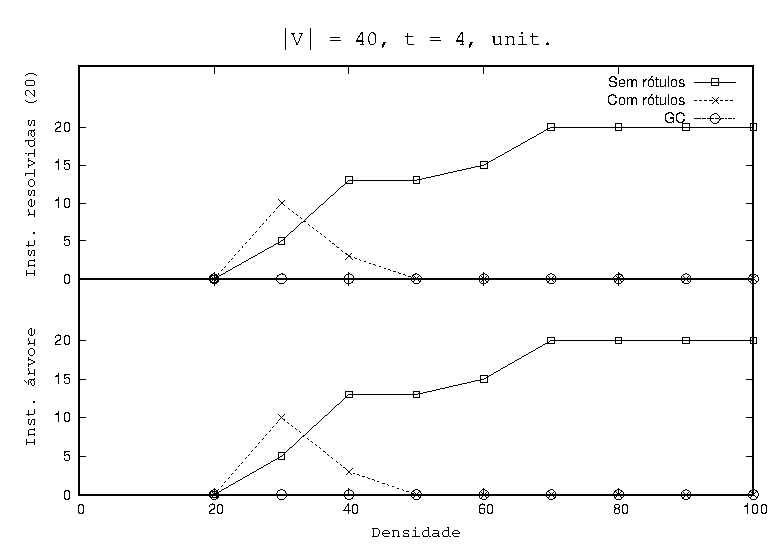
\includegraphics[scale=0.45]{figures/2inst_den-sf4-s40-unit}}%
    %\;
    \subfloat{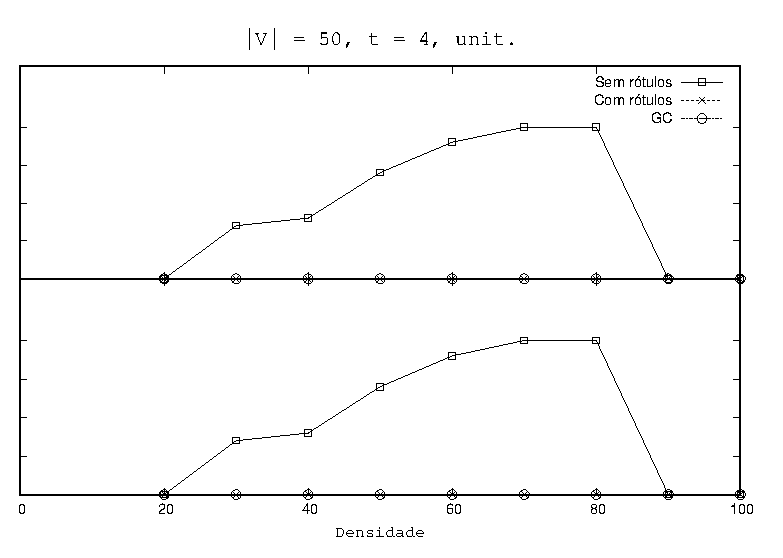
\includegraphics[scale=0.45]{figures/2inst_den-sf4-s50-unit}}
    \caption{}%
    \label{fig:tree_sf4_s40_50_unit}%
  \end{figure}

  \begin{itemize}
    \item Comportamento semelhante para $t = 3$
    \end{itemize}
\end{frame}

%% \begin{frame}{Quantidade de instâncias resolvidas para $t = 3$, peso unitário e ordem baixa}
%% \begin{figure}%
%%     \centering
%%     \subfloat{{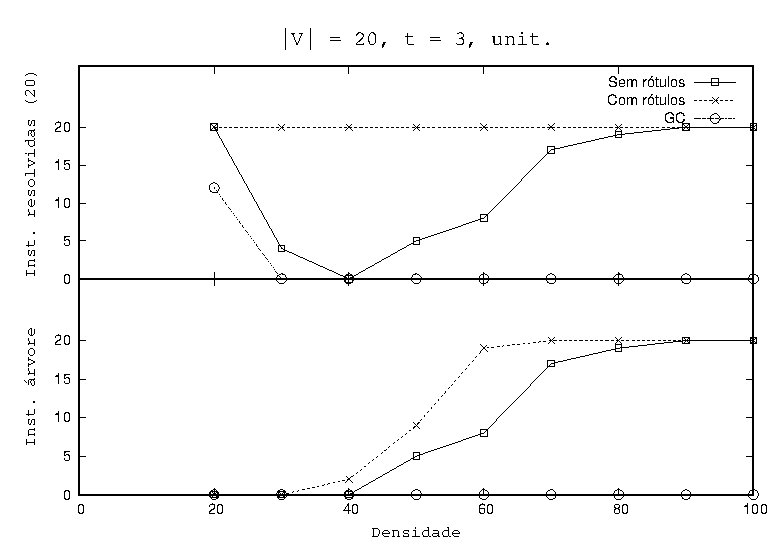
\includegraphics[scale=0.45]{figures/2inst_den-sf3-s20-unit} }}%
%%     %\;
%%     \subfloat{{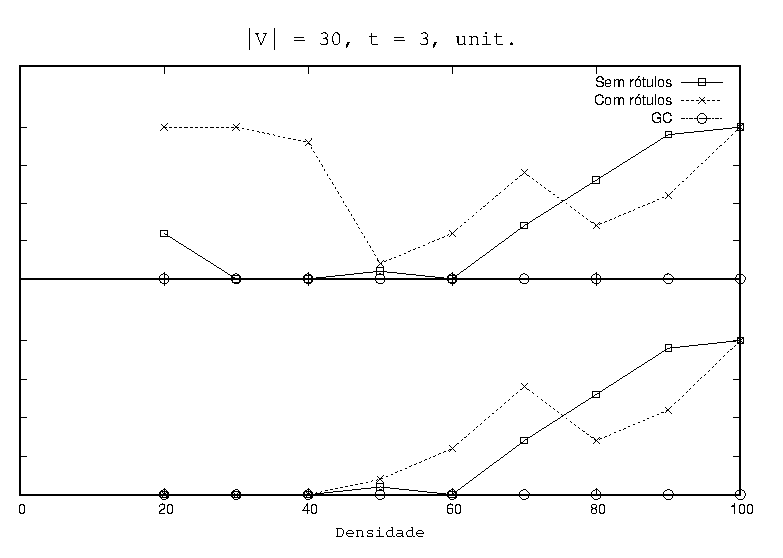
\includegraphics[scale=0.45]{figures/2inst_den-sf3-s30-unit} }}
%%     %% \caption{Quantidade de instâncias resolvidas para $t = 3$, peso unitário e ordem baixa}%
%%     \caption{}
%%     \label{fig:tree_sf3_s20_30_unit}%
%% \end{figure}
%% \begin{itemize}
%%   \item Para $t, |V|, den$ pequenos e peso unitário, $SR$ é melhor.
%%   \end{itemize}
%% \end{frame}

\begin{frame}{Quantidade de instâncias resolvidas}
\begin{figure}%
    \centering
    \subfloat{{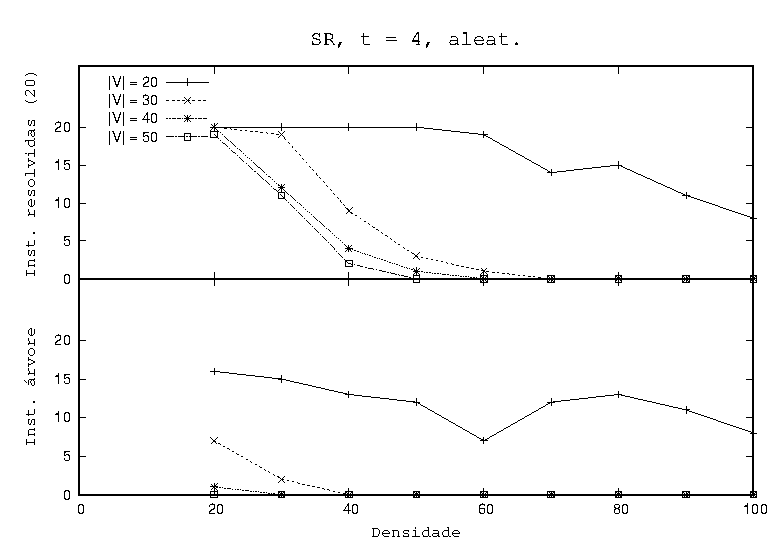
\includegraphics[scale=0.45]{figures/find-2inst_den-sf4-s20_50-random} }}%
    %\;
    \subfloat{{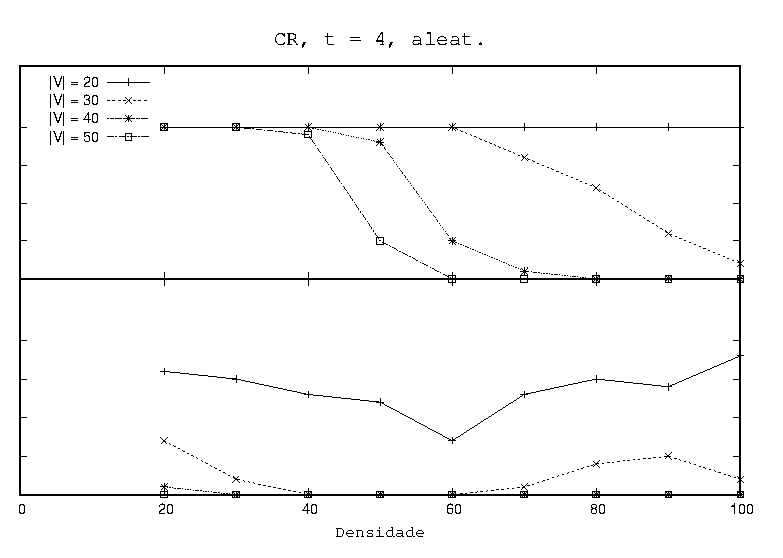
\includegraphics[scale=0.45]{figures/labels-2inst_den-sf4-s20_50-random} }}
    \caption{}%
    \label{fig:tree_sf4_s20_50_random}%
\end{figure}

\begin{itemize}
  \item Comportamento é semelhante para pesos aleatórios menos espaçados
  \end{itemize}
\end{frame}

%% \begin{frame}{Instâncias que admitem árvore $t$-spanner}
%%   \begin{itemize}
%%   \item Peso unitário:
%%     \begin{itemize}
%%     \item $t$ alto (ver Figura~\ref{fig:tree_sf4_s40_50_unit} e lado direito da
%%       Figura~\ref{fig:tree_sf3_s20_30_unit}).
%%     \end{itemize}
%%   \item Arestas com peso:
%%     \begin{itemize}
%%     \item $t$ alto.
%%       \item $|V|$ pequeno (ver Figura~\ref{fig:tree_sf4_s20_50_random}).
%%       \end{itemize}
    
%%   \end{itemize}  
%% \end{frame}

\begin{frame}{Maior tempo e ordem e menor $t$}
  \begin{itemize}
  \item <1->Maior tempo limite de execução
    \begin{itemize}
      \item <1->peso aleat. menos espaçado: CR e SR se comportam da mesma forma
    \end{itemize}
  \item <2->Valores maiores de ordem
    \begin{itemize}
      \item <2->peso aleat. menos espaçado: CR e SR se comportam da mesma forma
    \end{itemize}
  \item <3->Menor $t$
    \begin{itemize}
    \item <3->CR: todas as instâncias resolvidas em menos de $3s$
      \item <3->SR: tempo de execução bem maior
      \end{itemize}
    \end{itemize}
  \end{frame}

%% \begin{frame}{Maior tempo limite de execução}
%%   \begin{itemize}
%%   \item Peso aleatório menos espaçado:
%%     \begin{itemize}
%%     \item CR e SR se comportam de maneira semelhante quando o tempo limite é maior.
%%     \item Para $t = 3$, $|V| = 20$ ou $30$, todas as instâncias foram resolvidas por CR, exceto para $den = 20\%$.
%%     \item Para $t = 4$ e densidades altas, poucas instâncias resolvidas.
%%     \end{itemize}
%%   \end{itemize}
%% \end{frame}

%% \begin{frame}{Valores maiores de ordem}
%%   \begin{itemize}
%%     \item $60 \le |V| \le 80$
%%     \item Peso aleat. menos espaçado:
%%     \begin{itemize}
%%     \item CR e SR se comportam de maneira semalhante quando comparado ao tamanho menor de $|V|$.
%%       \begin{itemize}
%%         \item $> |V|, t, den \rightarrow $ $< \#$ inst. resolvidas.
%%         \end{itemize}
%%     \end{itemize}
%%   \item Peso unitário ($den = 20\%$):\\
%%     CR resolve poucas inst. para $t = 3$;\\
%%     SR resolve poucas inst. para $t = 4$.
%%     \end{itemize}
%% \end{frame}

%% \begin{frame}{Quantidade de instâncias resolvidas pela formulação CR para peso aleatório menos espaçado}
%% \begin{center}
%% \noindent
%% \footnotesize{
%% \begin{tabular}{|c|c|c|c|c|}\hline
%% {$t$} & {Densidade (\%)} & {Ordem} & {\# Inst. resolvidas} & {Tempo (s)}
%% \\ \hline\hline
%% \multirow{12}{*}{3}	&	20	&	60	&	10	&	$\num{1,3603393}$	\\
%% 	&	30	&	60	&	10	&	$\num{6,246502}$	\\
%% 	&	40	&	60	&	9	&	$\num{13,8250511111111}$	\\
%% 	&	50	&	60	&	0	&	0	\\
%% 	&	20	&	70	&	10	&	$\num{3,462295}$	\\
%% 	&	30	&	70	&	10	&	$\num{11,25421}$	\\
%% 	&	40	&	70	&	0	&	0	\\
%% 	&	50	&	70	&	0	&	0	\\
%% 	&	20	&	80	&	10	&	$\num{7,913799}$	\\
%% 	&	30	&	80	&	5	&	$\num{23,89124}$	\\
%% 	&	40	&	80	&	0	&	0	\\
%% &	50	&	80	&	0	&	0	\\
%% \hline
%% \multirow{3}{*}{4}	&	20	&	60	&	9	&	$\num{20,5626644444444}$	\\
%% 	&	20	&	70	&	7	&	$\num{66,0951857142857}$	\\
%% 	&	20	&	80	&	4	&	$\num{168,88825}$	\\
%% \hline\hline
%% \end{tabular}
%% }
%% \end{center}  
%%  \end{frame}

%% \begin{frame}{Fator de dilatação baixo}
%%   \begin{itemize}
%%     \item $t = \num{1,2}$ e $2$.
%%     \item CR: todas as instâncias resolvidas em menos de $3s$.
%%     \item SR:
%%       \begin{itemize}
%%       \item Tempo de execução bem maior.
%%         \item Instâncias não são resolvidas para $|V| = 50$ e $den \ge 80\%$.
%%         \end{itemize}
%%   \end{itemize}

%% \begin{figure}%
%%     \centering
%%     \subfloat{{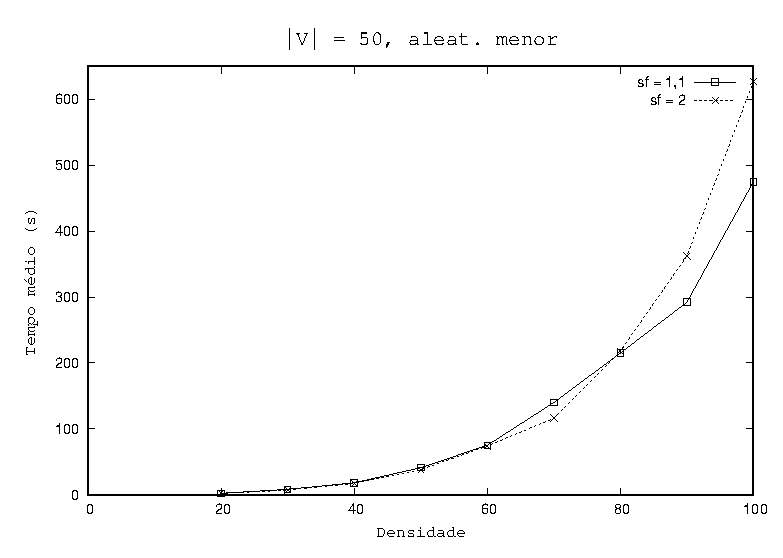
\includegraphics[scale=0.40]{figures/time_den-sf1_1-sf2-s50-small_random} }}%
%%     %\;
%%     \subfloat{{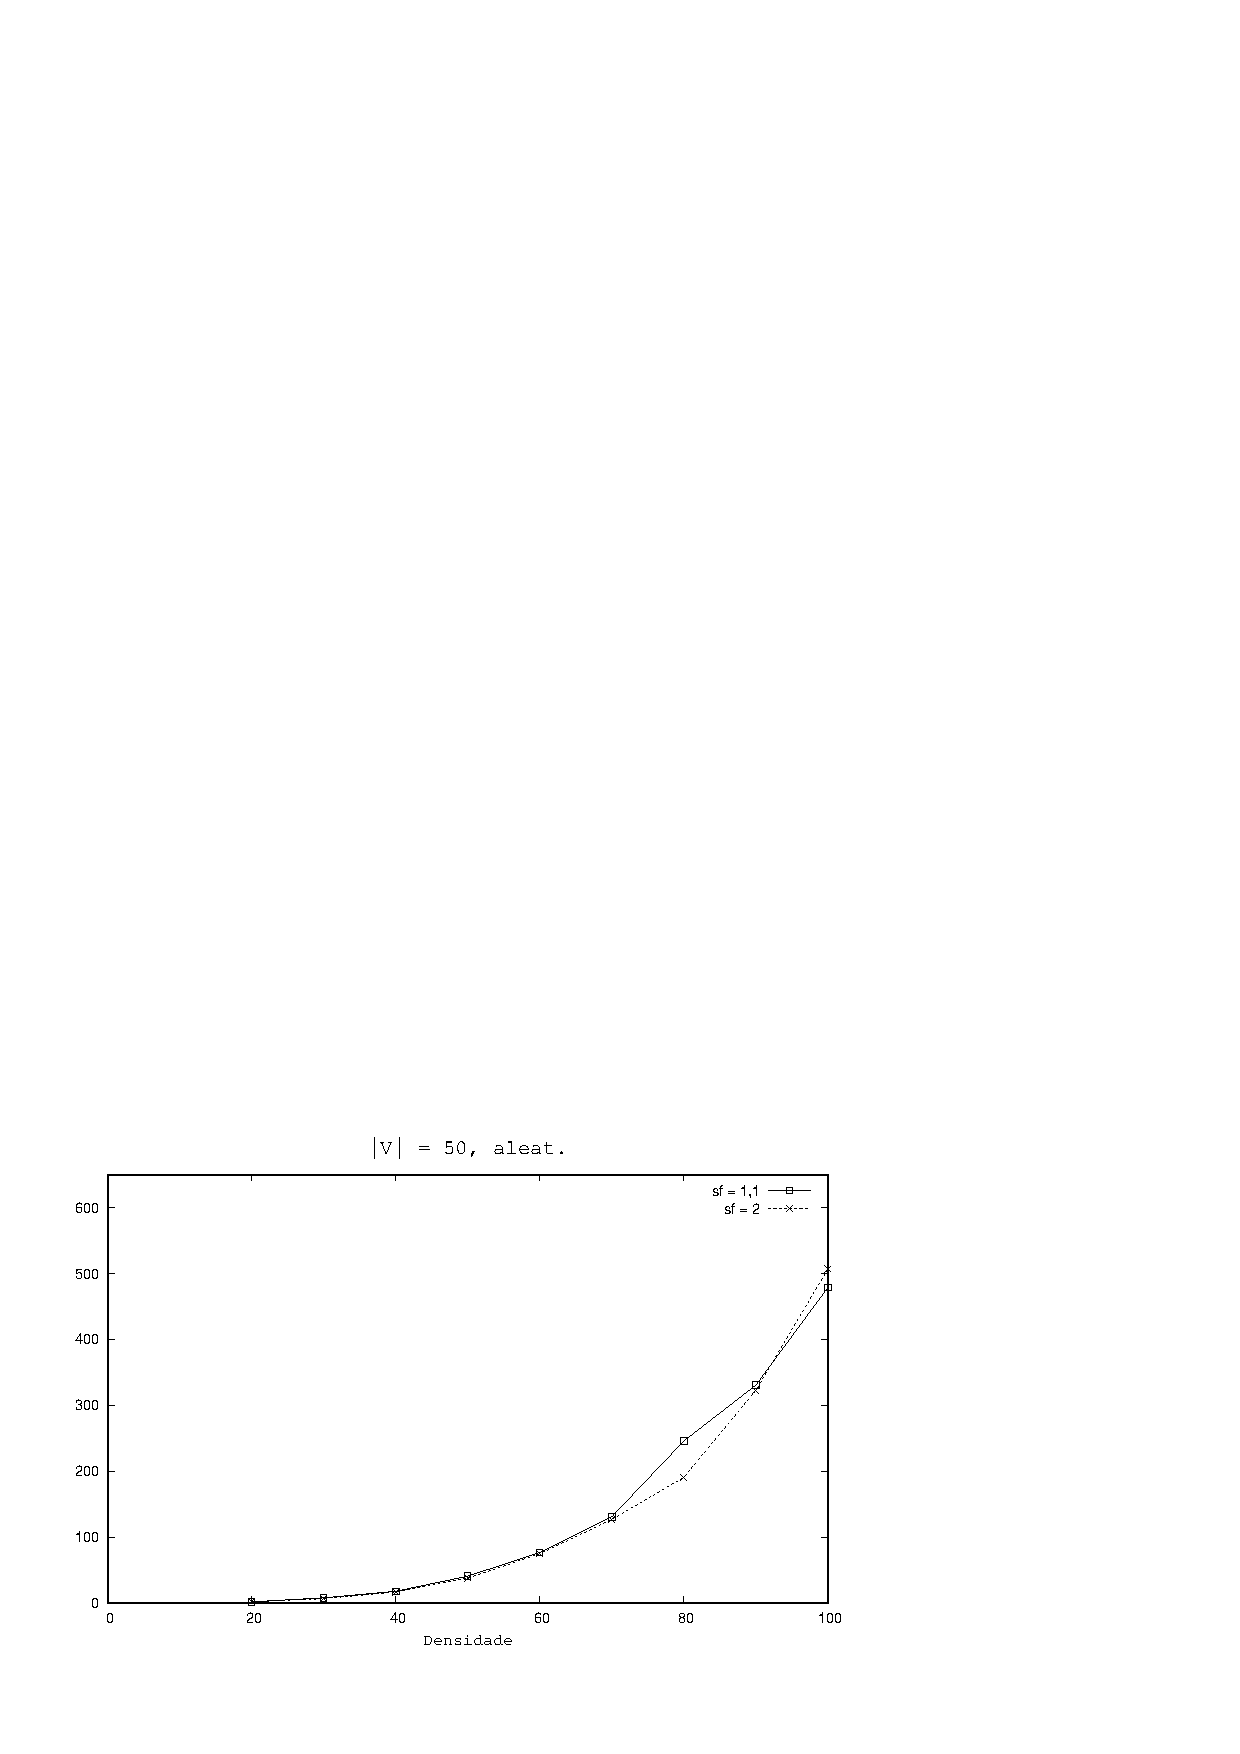
\includegraphics[scale=0.40]{figures/time_den-sf1_1-sf2-s50-random} }}    
%%     \label{fig:tree_sf1_1_sf2_s50_aleat}%
%% \end{figure}  
%%   \end{frame}

\begin{frame}{Recomendação de uso das formulações SR e CR}
%\scalebox{0.7}{
\begin{table}
  \centering
\scalebox{0.8}{
\begin{tabular}{llcccccc}
\toprule
& & \multicolumn{2}{c}{$t$ baixo} & \multicolumn{2}{c}{$t$ alto}\\
\cmidrule[0.05ex]{3-6}
& & P. unit. & P. aleat. & P. unit. & P. aleat. \\
\midrule[0.1ex]
Dens. alta & Ord. grande & SR & CR & SR & = \\ 
    &  Ord. peq. & SR (CR) & CR & CR & CR \\
\addlinespace
Dens. baixa & Ord. grande & CR & CR & SR & CR (SR) \\ 
    & Ord. peq. & CR & CR & CR (SR) & CR \\ 
\bottomrule
\end{tabular}
}
\end{table}
%}
  \end{frame}

\begin{frame}{Parte II}
  \begin{center}
    $t$-spanner de peso mínimo
  \end{center}
\end{frame}

\begin{frame}{Variando grau}
\begin{table}
  \centering
\scalebox{0.45}{
\begin{tabular}{|l|rrrrrr|rrrrrr|}
  %\toprule
  \hline
Grau & \multicolumn{6}{c|}{$4$} & \multicolumn{6}{c|}{$8$} \\
Ordem & 16 & 32 & 64 & 80 & 90 & 100 & 16 & 32 & 64 & 80 & 90 & 100 \\
\hline
\hline
$t = 1,1$ & $(10)$ & $(10)$ & $(10)$ & - & - & - & $(10)$ & $(10)$ & $(10)$ & - & - & -
\\ 
$t = 2$ & $(10)$ & $(10)$ & $(10)$ & - & - & - & $(10)$ & $(10)$ & $\num{6,408482} (10)$ & - & - & -
\\ 
$t = 3$ & $(10)$ & $(10)$ & $\num{10,1925287} (10)$ & $\num{7,824523} (10)$ & $\num{7,7401784} (10)$ & $\num{202,475267} (10)$ & $(10)$ & $\num{289,664214} (10)$ & $\num{133,767214285714} \;\,(7)$ & $\num{591,4651} \;\,(8)$ & $\num{371,9923} \;\,(6)$ & $\num{1146,8458} \;\,(5)$
\\
$t = 4$ & $(10)$ & $(10)$ & $\num{99,7693944444444} (10)$ & - & - & - & $\num{22,662389} (10)$ & $\num{709,6701} \;\,(6)$ & $\num{1157} \;\,(1)$ & - & - & -
\\
\hline
\end{tabular}
}
%% \caption{Instâncias resolvidas por GC e tempo de execução para peso aleatório}
\caption{Peso aleatório}
\label{tab:mwsp_random}
\end{table}


\begin{table}
  \centering
\scalebox{0.45}{
\begin{tabular}{|l|rrrrrr|rrrrrr|}
  \hline
Grau & \multicolumn{6}{c|}{$4$} & \multicolumn{6}{c|}{$8$} \\
Ordem & 16 & 32 & 64 & 80 & 90 & 100 & 16 & 32 & 64 & 80 & 90 & 100 \\
\hline
\hline
$t = 1,1$ & $(10)$ & $(10)$ & $(10)$ & - & - & - & $(10)$ & $(10)$ & $(10)$ & - & - & -
\\ 
$t = 2$ & $(10)$ & $(10)$ & $(10)$ & - & - & - & $(10)$ & $(10)$ & $\num{5,387807} (10)$ & - & - & -
\\
$t = 3$ & $(10)$ & $(10)$ & $(10)$ & $\num{5,2910455} (10)$ & $(10)$ & $\num{7,7604249} (10)$ & $(10)$ & $\num{49,224839} (10)$ & $\num{675,009777777778} \;\,(9)$ & $\num{744,797222222222} \;\,(9)$ & $\num{596,4886} (10)$ & $\num{667,042375} \;\,(8)$
\\
$t = 4$ & $(10)$ & $\num{6,1226376} (10)$ & $\num{312,173572} (10)$ & - & - & - & $\num{163,913996} (10)$ & $\num{1708,26471428571} \;\,(7)$ & $0$ & - & - & -
\\
\hline
\end{tabular}
}
%% \caption{Instâncias resolvidas por GC e tempo de execução para distância euclidiana}
\caption{Distância euclidiana}
\label{tab:mwsp_euclidean}
\end{table}
\end{frame}

\begin{frame}{Resultados}
  \begin{itemize}
  \item Variando grau:
    \begin{itemize}
    \item Com peso:\\
      $t = 2$: GC é melhor com distância euclidiana\\
      $t = 3$: GC é melhor com distância euclidiana\\
      $t = 4$: GC é melhor com pesos aleatórios
    \end{itemize}
  \item <2->Variando densidade:
    \begin{itemize}
      \item <2->Sem peso:\\
        $t = 2$: GC é melhor com distância euclidiana\\
        $t = 3$: GC é melhor com pesos aleatórios\\
        $t = 4$: GC é melhor com pesos aleatórios
      \end{itemize}
    \end{itemize}
  \end{frame}

%% \begin{itemize}
%% \item Peso aleat:
%%   \begin{itemize}
%%   \item $t = 3$: tempo bem maior para $|V| \ge 100$.
%%   \end{itemize}
%% \item Dist. euclidiana:
%%   \begin{itemize}
%%   \item $t = 3$: escala bem para grau~4; para grau~8, admite-se ordens maiores.
%%   \item $t = 4$: GC se comporta melhor neste cenário quando comparado com os pesos aleatórios.
%%   \end{itemize}
%% \end{itemize}  
%% \end{frame}

%% \begin{frame}{Variando densidade}
%% \begin{figure}%
%%     \centering
%%     \subfloat{{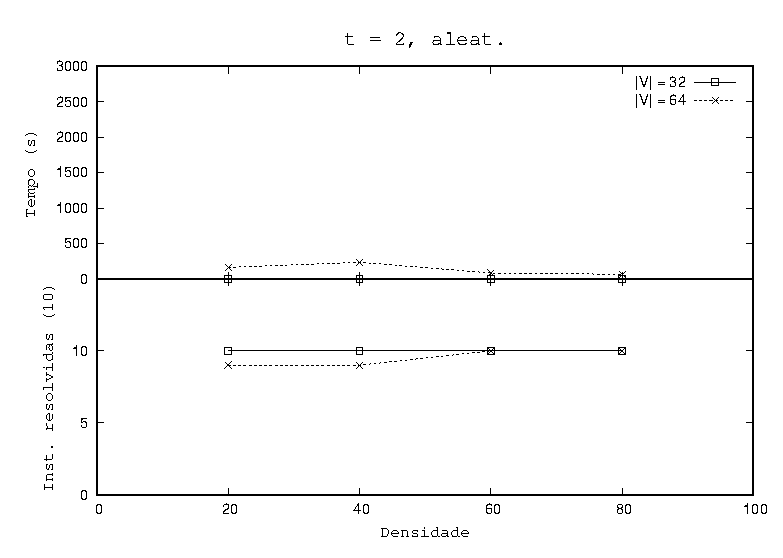
\includegraphics[scale=0.35]{figures/time_inst_den-sf2-random} }}%
%%     %\;
%%     \subfloat{{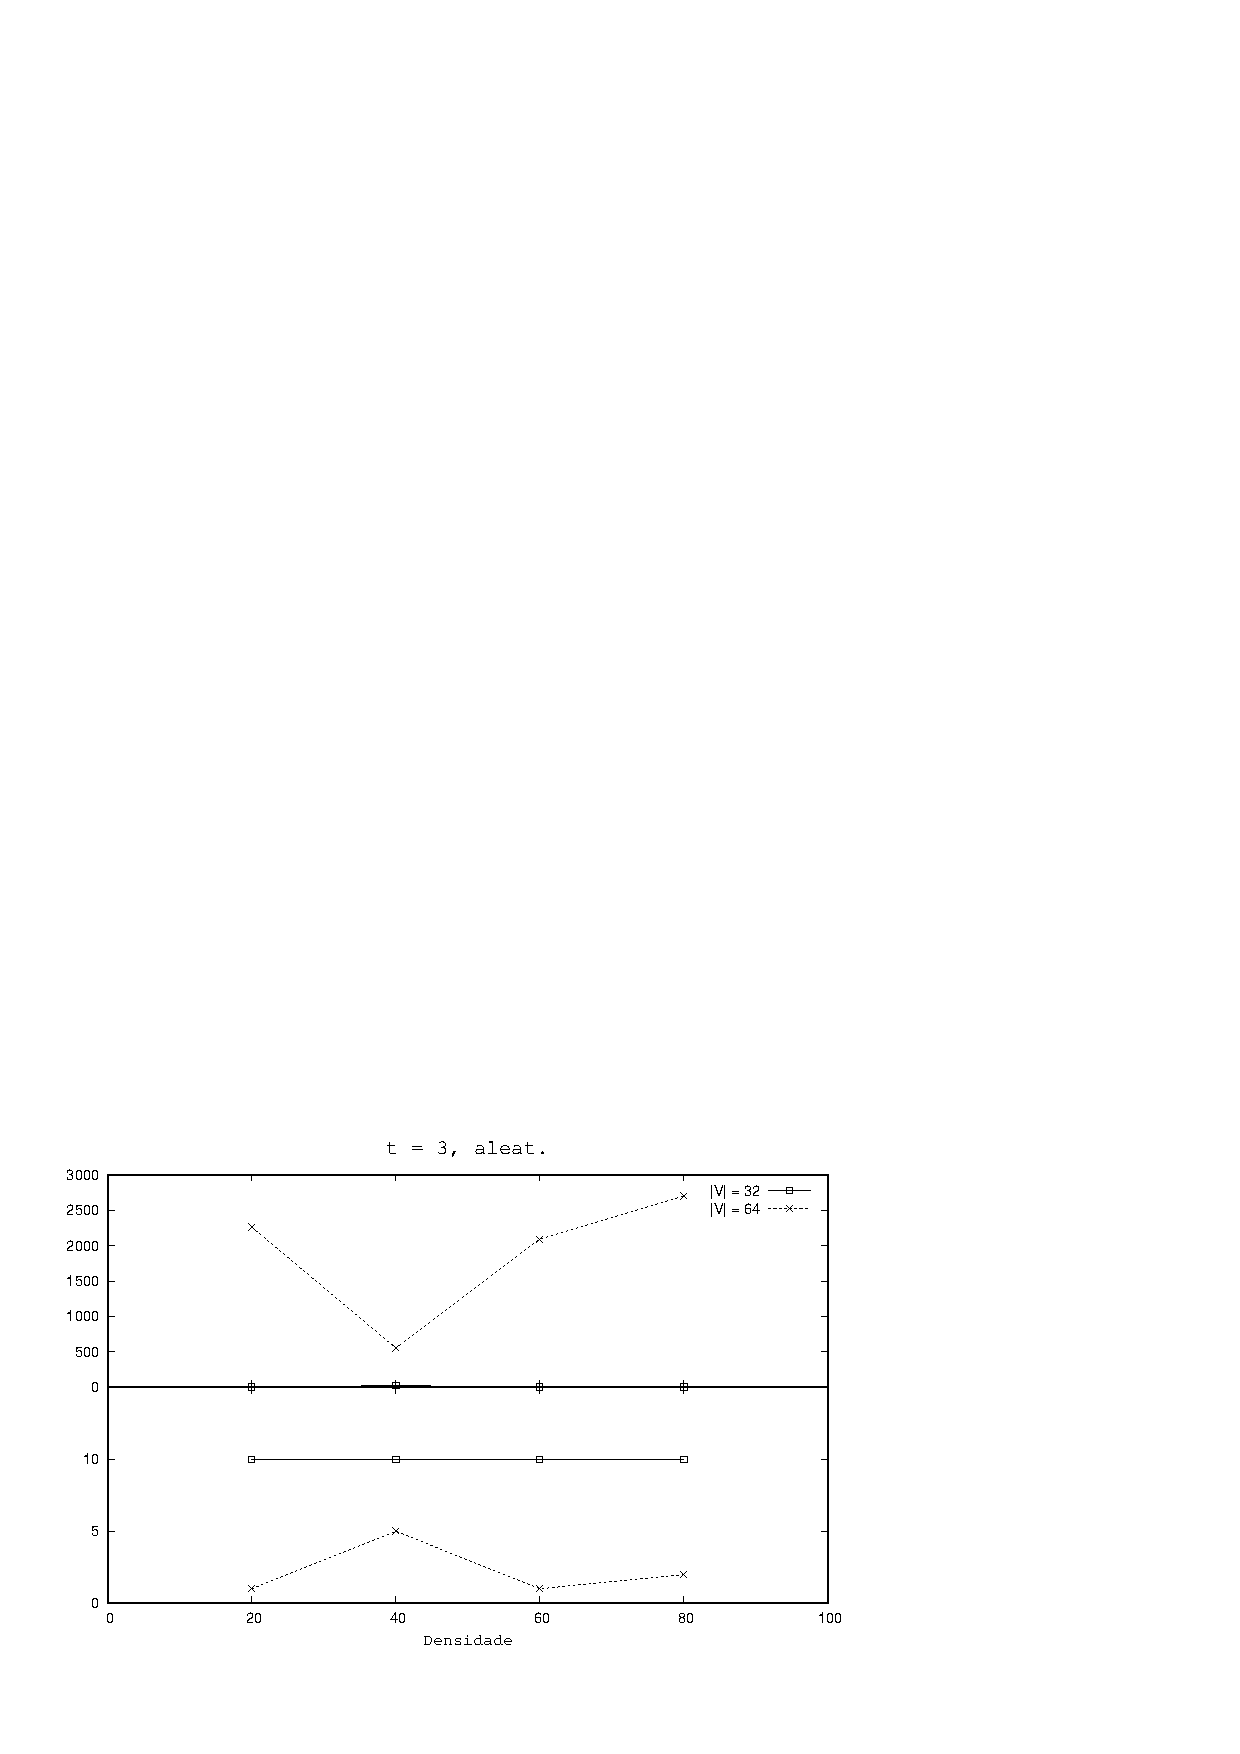
\includegraphics[scale=0.35]{figures/time_inst_den-sf3-random} }}    
%%     \label{fig:time_inst_den-sf2_sf3-random}%
%% \end{figure}

%% \begin{figure}%
%%     \centering
%%     \subfloat{{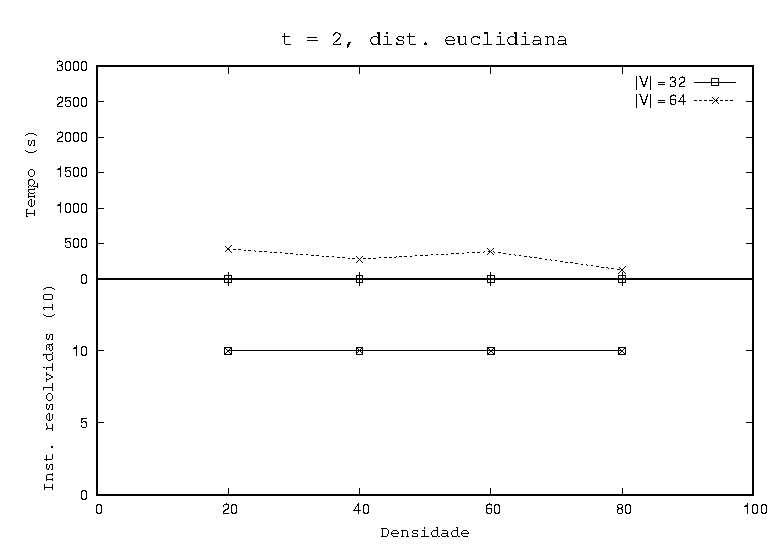
\includegraphics[scale=0.35]{figures/time_inst_den-sf2-euclidean} }}%
%%     %\;
%%     \subfloat{{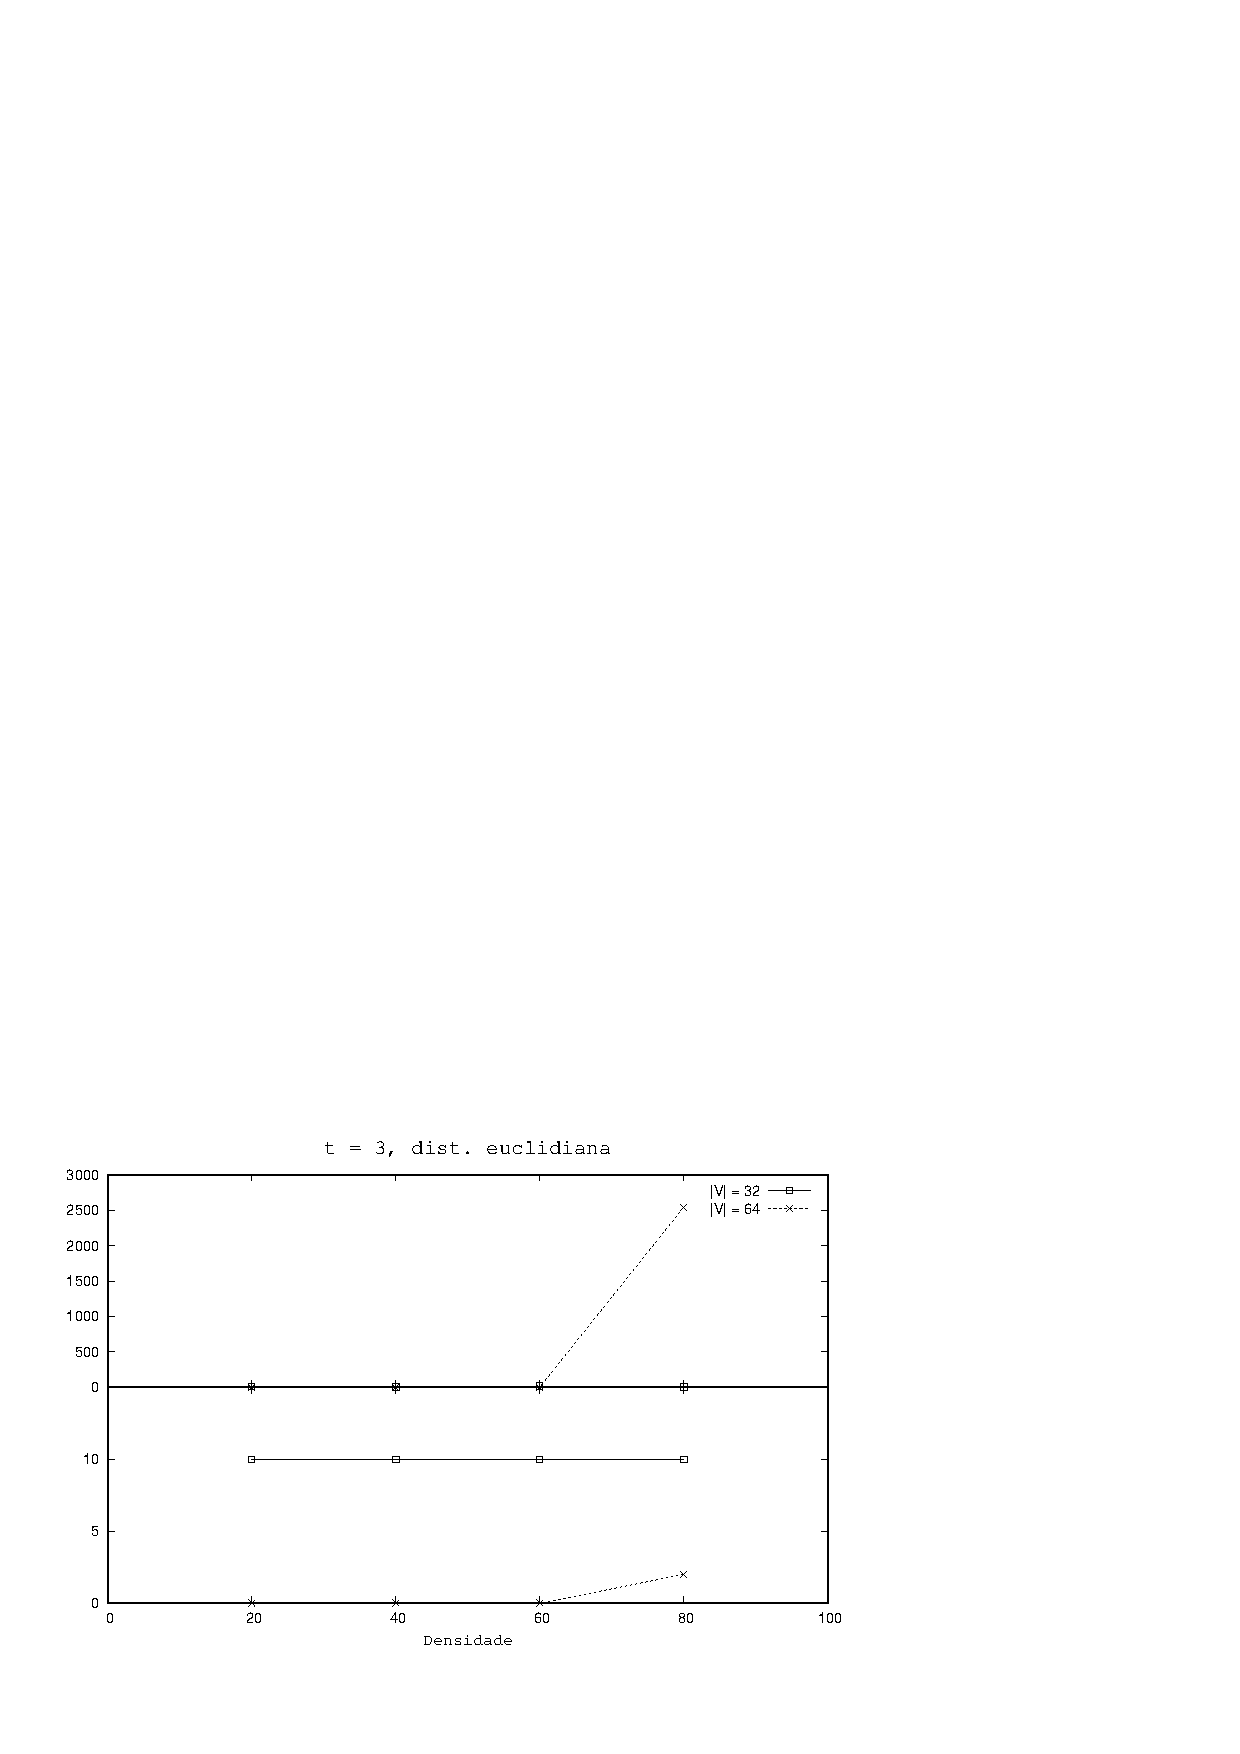
\includegraphics[scale=0.35]{figures/time_inst_den-sf3-euclidean} }}    
%%     \label{fig:time_inst_den-sf2_sf3-euclidean}%
%% \end{figure}
%% \end{frame}

%% \begin{frame}{Variando densidade}
%% \begin{itemize}
%% \item Ambos os pesos:
%%   \begin{itemize}
%%   \item $t = 2$: resolve quase todas instâncias.
%%   \item $t = 3$: muito menos instâncias são resolvidas quando $|V|$ aumenta de 32 para 64.
%%   \item GC é melhor com o peso aleatório.
%%   \end{itemize}
%%   \item Caso unitário: $> t, |V| \rightarrow < \#$ inst. resolvidas.
%% \end{itemize}  
%%   \end{frame}

%% \begin{frame}{Outros dados}
%% \begin{figure}%
%%     \centering
%%     \subfloat{{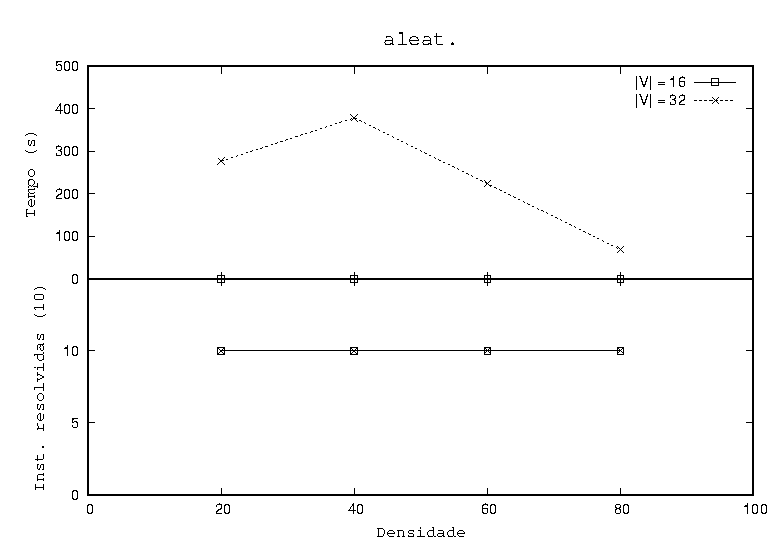
\includegraphics[scale=0.40]{figures/time_inst_den-sf4-random} }}%
%%     %\;
%%     \subfloat{{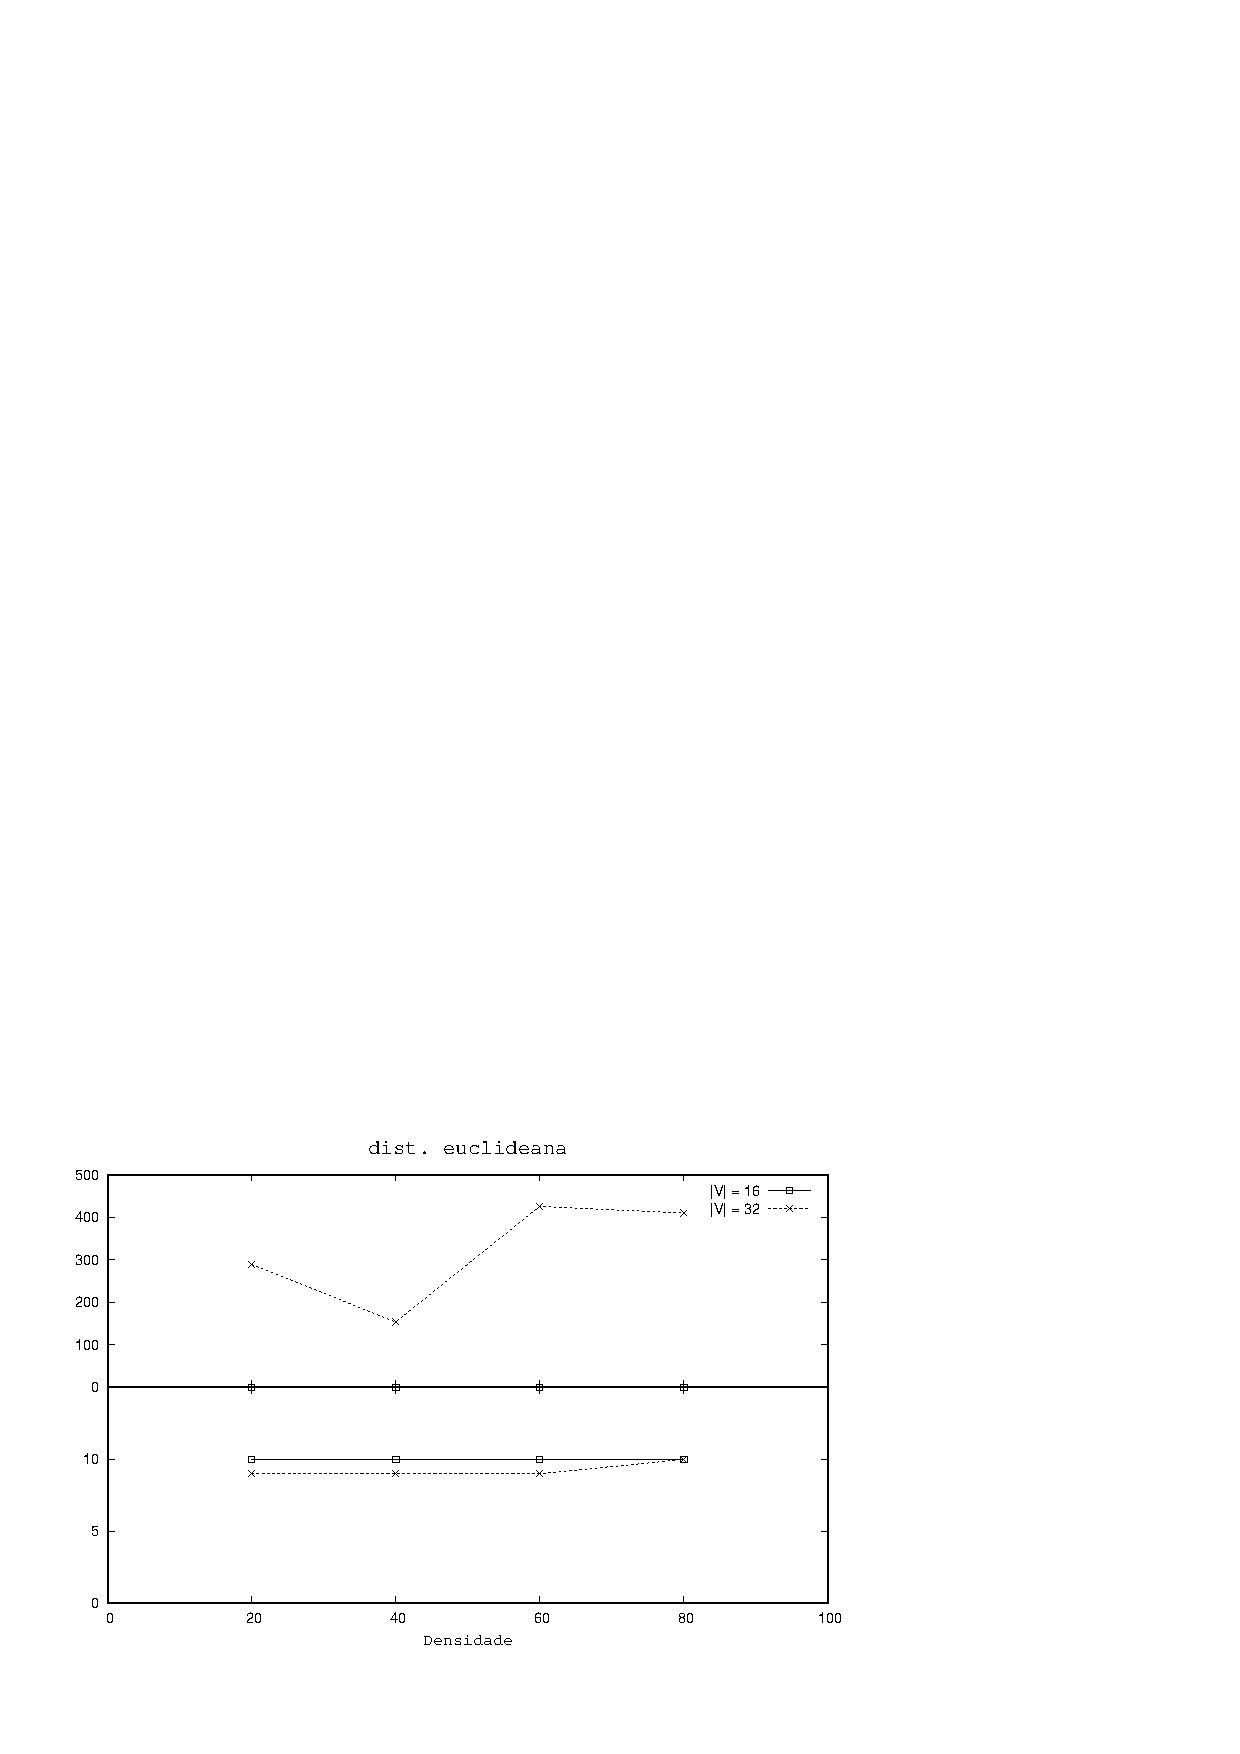
\includegraphics[scale=0.40]{figures/time_inst_den-sf4-euclidean} }}    
%% \end{figure}
  
%%   \begin{itemize}
%%   \item Para $t = 4$, $|V| = 32$ e peso aleatório: curva apresenta
%%     comportamento de decaimento.
%%   \item Peso unit.: $> t, |V| \rightarrow < \#$ inst. resolvidas.
%%     \item Em geral: $> t, den \rightarrow > \#$ sol. viáveis.
%%     \end{itemize}
%%   \end{frame}

\begin{frame}{}
  \begin{center}
    Obrigado
    \end{center}
  \end{frame}

\appendix

\begin{frame}{Histórico \hyperlink{hist}{\beamergotobutton{$\leftarrow$}}}
  \hypertarget{histmaior}{}
  \begin{itemize}    
  \item <1-> 1992 - 1995: resultados clássicos de complexidade.
  \item <2-> 1993 - 2001: classes específicas de grafos.
  \item <3-> 2001 - 2008: (in)aproximabilidade para classes gerais.
  \item <4-> 2009 - 2014: algoritmos de aproximação baseados em PL.
  \item <5-> 2015 - 2018: spanners distribuídos, oráculos de distância e
    spanners esparsos.    
  \end{itemize}
\end{frame}


\begin{frame}{Definições equivalentes de spanner \hyperlink{span}{\beamergotobutton{$\leftarrow$}}}
  \hypertarget{defspan}{}
  \begin{itemize}
    \item Afirmações equivalentes:
      \begin{itemize}
        \item[{\rm (a)}] $H$ é um $t$-spanner de $G$, isto é, $H$ satisfaz (\ref{eq:def_spanner});
        \item[{\rm (b)}] $\dist_{H}(u,v) \le t \cdot \dist_{G}(u,v) \;\forall\,uv \in E$;
        \item[{\rm (b')}] $\dist_{H}(u,v) \le t \cdot \dist_{G}(u,v) \;\forall\,uv \in E \setminus E(H)$;
        \item[{\rm (c)}] $\dist_{H}(u,v) \le t \cdot w_{uv} \;\forall\,uv \in E$.
        \item[{\rm (c')}] $\dist_{H}(u,v) \le t \cdot w_{uv} \;\forall\,uv \in E \setminus E(H)$.
        \end{itemize}
    \end{itemize}
\end{frame}

\begin{frame}{Significado da variável $y$ \hyperlink{form_1}{\beamergotobutton{$\leftarrow$}}}
  \hypertarget{sig_y}{}
  {\footnotesize
  \begin{itemize}
    \item $\forall u,v \in V$, seja $T_{u,v}$ o caminho entre $u$ e $v$ em $T$.
    \item $\forall uv,ij \in E$:
  \end{itemize}
\begin{align*}
  d^{u v}_{ij} := z^{u}_{ij} - z^{v}_{ij}\\
  s^{u v}_{ij} := z^{u}_{ij} + z^{v}_{ij}\\
  \end{align*}

%\small
\begin{center}
  \noindent
  %\captionof{table}{Diferenças e somas relativas à variável $z$}
  \label{tab:sum_diff} 
\begin{tabular}{|r|r|r|r|}\hline
{$d^{uv}_{ij}$ $s^{uv}_{ij}$} & {$z^{u}_{ij}$ $z^{v}_{ij}$} & {$z^{u}_{ji}$ $z^{v}_{ji}$} & {$d^{uv}_{ji}$ $s^{uv}_{ji}$}
\\ \hline\hline 
$1\quad 1$ & $1\quad 0$ & $0\quad 1$ & $-1\quad 1$ \\
$-1\quad 1$ & $0\quad 1$ & $1\quad 0$ & $1\quad 1$ \\
$0\quad 2$ & $1\quad 1$ & $0\quad 0$ & $0\quad 0$ \\
$0\quad 0$ & $0\quad 0$ & $1\quad 1$ & $0\quad 2$ \\
$0\quad 0$ & $0\quad 0$ & $0\quad 0$ & $0\quad 0$ \\
\hline\hline
\end{tabular}
\end{center}


\begin{lpformulation}[]
  \lpeq[res_mwstp:define_y_ij]{d^{uv}_{ij} \le y^{uv}_{e} \le s^{uv}_{ij}} {uv \in E, \forall e = \{i,j\} \in E}
  \lpeq[res_mwstp:define_y_ji]{d^{uv}_{ji} \le y^{uv}_{e} \le s^{uv}_{ji}} {uv \in E, \forall e = \{i,j\} \in E}
\end{lpformulation}

\begin{align}
  \label{afirm:valor_y}
  y^{uv}_e = 1 \Leftrightarrow e \in T_{u,v}.
\end{align}
}

\end{frame}

\begin{frame}{Significado da variável $u^{r}$ \hyperlink{var_u}{\beamergotobutton{$\leftarrow$}}}
  \hypertarget{sig_u}{}

\begin{figure}[t]
  \centering
  \scalebox{0.7}{
\begin{tikzpicture}%
  [>=stealth,
   %shorten >=1pt,
   node distance=2cm,
   %% scale=0.6, every node/.style={scale=0.6},
   %% on grid,
   auto%,
%   every state/.style={draw=black!60, fill=black!5, very thick}
  ]

\tikzset{myptr/.style={decoration={markings,mark=at position 0.5 with %
      {\arrow[scale=2,>=stealth]{>}}},postaction={decorate}}}
  
  
          \tikzstyle{every state}=[
            draw = black,
            thick,
            fill = white,
            minimum size = 4mm
        ]
  
\node[state] (l1) [label=right:$r$]                  {};
\node[state] (l2) [label=above:$i$, below left of=l1] {};
\node[state] (l3) [below right of=l1] {};
\node[state] (l4) [label=below:$j$, below left of=l2] {};
%\node[state] (l5) [label=right:$b_1$,below right of=l2] {};
\node[state] (l5) [below right of=l2] {};
\node[state] (l6) [below right of=l3] {};
\node[state] (l7) [below left of=l5] {};
\node[state] (l8) [below right of=l5] {};
\node[left] at (l4.west){$T^{r}$:};

\path[]
%   FROM       BEND/LOOP           POSITION OF LABEL   LABEL   TO
   (l1)     edge[bend left, myptr]     node                    {} (l2)
    (l3)   edge[bend left, myptr]     node                    {} (l1)
(l2)    edge[bend left, myptr]     node                    {} (l4)
(l4)    edge[dotted, bend left, myptr]     node                    {$z^{r}_{ji} = 0$} (l2)
    (l3)    edge[bend left, myptr]     node                    {} (l5)
    (l6)    edge[bend left, myptr]     node                    {} (l3)
    (l5)    edge[bend left, myptr]     node                    {} (l8)
    (l4)    edge[bend left, myptr]     node                    {} (l7)
   ;
\end{tikzpicture}
}
  \label{fig:variavel_u}
\end{figure}
  
  {\footnotesize
  \begin{itemize}

  \item Ineq. \ref{res:mtz_var} com relação ao arco $ij:$
    \begin{align*}
  u^{r}_i - u^{r}_j + (M^{r}_{ij} + w_{ij}) \cdot 1 + (M^{r}_{ij} - w_{ij}) \cdot 0 \le M^{r}_{ij} \Rightarrow u^{r}_j \ge u^{r}_i + w_{ij}.
\end{align*}
    
  \item Ineq. \ref{res:mtz_var} com relação ao arco $ji:$
    \begin{align*}
  u^{r}_j - u^{r}_i + (M^{r}_{ji} + w_{ij}) \cdot 0 + (M^{r}_{ji} - w_{ij}) \cdot 1 \le M^{r}_{ji} \Rightarrow u^{r}_j \le u^{r}_i + w_{ij}.
\end{align*}

\begin{align*}
  u^{r}_j = u^{r}_i + w_{ij}.
\end{align*}

    
  \end{itemize}
}
  
\end{frame}

\begin{frame}{Heurística primal \hyperlink{heurprimal}{\beamergotobutton{$\leftarrow$}}}
  \hypertarget{heurcluster}{}
  \scalebox{0.7}{
    \begin{algorithm}[H]
      \SetAlgoLined
      \Input{$G=(V, E)$, onde $|V|=n$, e um inteiro positivo $k$}
      \Output{partição $\partition$ de $V$}
      \BlankLine  
      $\partition \gets \emptyset$\;
      Seja $G'=(V',E')$ um grafo isomorfo a $G$\;
      \While{$V' \neq \emptyset$}{
        Selecione um vértice arbitrário $v' \in V'$\;
        $S' \gets \{v'\}$\;
        \While{$|\verneigh(S')| < n^{1/k}|S'|$}{
          $S' \gets \verneigh(S')$\;
        }
        Seja $S = \{v \in V\;|\; \exists\; v' \in S' \text{ t.q. } v' \text{ é o vértice correspondente a } v \text{ no isomorfismo}\}$\;
        $\partition \gets \partition \cup \{S\}$\;
        $V' \gets V' \setminus S'$\;
      }
      \caption{Partição básica} 
      \label{alg:basic_part}
    \end{algorithm}
    }
  \end{frame}

  \begin{frame}{Heurística primal \hyperlink{heurprimal}{\beamergotobutton{$\leftarrow$}}}
    \scalebox{0.7}{
    \begin{algorithm}[H]
      \LinesNumbered
      %% \SetAlgoLined
      \Input{$G=(V,E)$, inteiro positivo $k$}
      \Output{Um grafo $G'=(V,E')$ que é um $(2k-1)$-spanner de $G$ com no máximo $O(n^{1 + 1/k})$ arestas}
      \BlankLine
      Construir uma partição $\partition$ de $V$ usando o Algoritmo~\ref{alg:basic_part} (Partição básica)\;

      \ForEach{$S_i \in \partition$}{
        $T_i$ $\gets$ uma árvore de caminhos mínimos de $G[S_i]$
        enraizada em algum vértice;
      }
      $E' \gets \bigcup_{S_i \in \partition}E(T_i)$\;
      $\breve{E} \gets \emptyset$\;
      \ForEach{$S_i \in \partition$}{
        \ForEach{$v \in \verneigh(S_i) \setminus S_i$}{
          Seja $u \in S_i$ t.q. $uv \in E$\;
          $\breve{E} \gets \breve{E} \cup uv$\;
        }
      }
      $E' \gets E' \cup \breve{E}$\;
      \caption{Spanner baseado em partição em clusters} 
      \label{alg:unweighted_span}
    \end{algorithm}
    }
  \end{frame}

  \begin{frame}{Spanner baseado em partição de clusters \hyperlink{heurprimal}{\beamergotobutton{$\leftarrow$}}}    
\begin{teorema}
  O Algoritmo~\ref{alg:unweighted_span} aplicado a um grafo $G$ de
  ordem $n$, e um inteiro positivo~$k$,  constrói um $(2k-1)$-spanner de
  $G$ com no máximo $O(n^{1+1/k})$ arestas.
  \end{teorema}
    \end{frame}

  \begin{frame}{Outra heurística primal \hyperlink{heurprimal}{\beamergotobutton{$\leftarrow$}}}
\hypertarget{heurguloso}{}
\begin{algorithm}[H]
  \SetAlgoLined
  \Input{$G=(V, E)$ com pesos não-negativos nas arestas, real $t \ge 1$}
  \Output{$t$-spanner $G'$ de $G$ com peso pequeno}
  \BlankLine
  Ordene as arestas de $E$ em ordem não-decrescente de seus pesos\;
  $G' \gets (V,E')$, onde $E'= \emptyset$\;
  \ForEach{$e=uv \in E$}{
    \lIf{$t \cdot w(e) < \dist_{G'}(u,v)$}{$E'$ $\gets$ $E' \cup e$}
  }
  \caption{Algoritmo Guloso de Althöfer et al.} 
  \label{alg:greedy_spanner}
\end{algorithm}

  \end{frame}

  \begin{frame}{Heurística dual \hyperlink{heurdual}{\beamergotobutton{$\leftarrow$}}}
    \hypertarget{heurmst}{}
    \scalebox{0.7}{
      \begin{algorithm}[H]
        \SetAlgoLined
        \Input{$G=(V,E)$, $E_0 \subset E$, $E_1 \subset E$, $w: E \to \mathbb{R}^+$}
        \Output{: limitante dual para a tripla $(G,E_0,E_1)$}
        /* $E_0$: conjunto das arestas fixadas em $0$; $E_1$: conjunto das arestas fixadas em $1$. */ 
        \BlankLine
        $LD \gets \sum_{e\in E_1}w(e)$\;  
        Seja $G_1=(V,E_1)$, e $\comp$ o conjunto dos componentes de $G_1$\;
        Seja $G_{1}^{c} = (V^c_1,E^c_1)$ o grafo assim definido:\\
        $~~ V^c_1 = \{C_i | \; C_i \in \comp\}$\;
        $~~ E^c_1 = \{C_iC_j \; | \; C_i,C_j \in \comp, i \neq j,  \text{ e } \exists x,y \in V(G) \text{ t.q. } x \in V(C_i), y \in V(C_j), xy \in E(G), xy \notin E_0\}$\;
        $T \gets {\rm MST}(G^c_1)$\; 
        $LD \gets LD + \sum_{e \in E(T)}w(e)$\;
        \Return $LD$.   
        \BlankLine 
        \caption{MST baseada nas arestas fixadas pelo B\&B} 
        \label{alg:mst_based_fixed_edges}
      \end{algorithm}
    }
  \end{frame}

  \begin{frame}{Custo reduzido \hyperlink{dualrelax}{\beamergotobutton{$\leftarrow$}}}
    \hypertarget{provacustoreduzido}{}
    \begin{teorema}
      Considerede $x$ uma solução viável básica associada a uma matrix base $B$,
      e seja $\tilde{c}$ o vetor custo reduzido correspondente.
      Se $\tilde{c} \ge 0$, então $x$ é ótima.
      \end{teorema}
  \end{frame}

  \begin{frame}{CSPP \hyperlink{pricing}{\beamergotobutton{$\leftarrow$}}}
\hypertarget{cspp}{}    
  \scalebox{0.6}{
\begin{algorithm}[H]
  \SetAlgoLined
  \Input{$G=(V, E)$, $w: E \to \mathbb{Z}^+$, $c: E \to \mathbb{Z}^+$, real $B$, real $M$, $s \in V$, $d \in V$}
  \Output{caminho $p_f$ entre $s$ e $d$ de menor custo satisfazendo a restrição de peso máximo $B$ e de custo máximo $M$}
  \BlankLine
  $p_f \gets null$\;
  Calcula as árvores de caminhos de peso e custo mínimos $T^w$ e $T^c$\;
  $H \gets \{(\{\},s,0,0)\}$\;
  \While{$H \neq \emptyset$}{
    Escolha o rótulo $(p,n,w,c)$ mais barato (em termos de custo) no conjunto $H$\;
    \If{$n = d$}{
      $p_f \gets p$\;
      \Return $p_f$.
    }
    \ForEach{$n_i \in \neigh_{G}(n)$}{
      Seja $e_i = nn_i$.
      Crie o novo rótulo $(p \cup \{e_i\}, n_i, w + w_{e_i}, c + c_{e_i})$\;
      Descarte todos os novos rótulos tal que $w + w_{e_i} + T^{w}(n_i) > B$ ou
      $c + c_{e_i} + T^{c}(n_i) > M$. Para os demais, armazene em $H$\;
      Descarte (de $H$) rótulos dominados\;
    }
    \Return $p_f$.
  }
  \caption{CSPP} 
  \label{alg:cspp}
\end{algorithm}
  }
  \end{frame}
  

\begin{frame}{Solução viável sem suporte minimal \hyperlink{formmwsp}{\beamergotobutton{$\leftarrow$}}}
\hypertarget{supminimal}{}
\begin{figure}[t] 
  \centering
  \scalebox{0.7}{  
    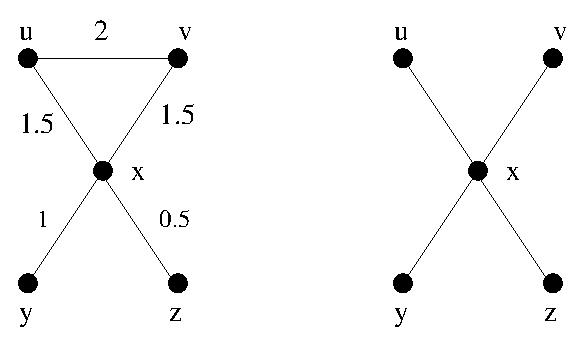
\includegraphics[scale=0.45]{figures/exemplo_Y_minimal}
    }
\caption{Um grafo $G$ com seu respectivo 2-spanner ($H$) de peso mínimo}
\label{fig:exemplo_Y_minimal}
\end{figure}

\begin{itemize}
  \item Para cada $e = pq, f \in E$, defina:
\end{itemize}

\begin{align*}
x^*(e) &= \incid^{H}_{e},\\
Y^*(e,f) &= 
\begin{cases}
    1& \text{se $f \in E(H_{p,q}),$}\\
    1& \text{se $e = xy, f = xz,$}\\
    0& \text{caso contrário.}
    %% 0& \text{se $f \in E \setminus E(H_{p,q}).$}
\end{cases}
\end{align*}

\begin{itemize}
\item $(x^*,Y^*)$ é uma sol. ótima t.q. $Y^*$
  não tem sup. minimal.
\end{itemize}

  \end{frame}
  

  \begin{frame}{Prova \hyperlink{dualrelax}{\beamergotobutton{$\leftarrow$}}}
    \begin{proof}
      \begin{itemize}
      \item <1-> Seja $y$ uma sol. viável qualquer e defina $d = y - x$.
      \item <2-> $x$ e $y$ são viáveis $\Rightarrow$ $Ax = Ay = b$ e $Ad = 0$.
      \item <3-> $Ad = Bd_{B} + \sum_{i \in N} A_{i}d_{i} = 0$.
      \item <4-> $B$ é inversível $\Rightarrow$ $d_{B} = - \sum_{i \in N} B^{-1}A_{i}d_{i}$.
      \item <5-> $cd = c_{B}d_{B} + \sum_{i \in N}c_{i}d_{i} = \sum_{i \in N}(c_i - c_{B}B^{-1}A_{i})d_i = \sum_{i \in N} \tilde{c_i}d_i$.
      \item <6-> $x_i = 0$ ($x$ é sol. bás. viável) e $y_i \ge 0$ ($y$ é viável) $\forall i \in N$.
      \item <7-> Então $d_i = y_i - x_i \ge 0, \forall i \in N$.
      \item <8-> $\tilde{c_i} \ge 0$ (por hipót.) $\forall i \in N \Rightarrow \tilde{c_i}d_i \ge 0 \forall i \in N$.
      \item <9-> $c(y - x) = cd = \sum_{i \in N} \tilde{c_i}d_i$.
        \item <10-> Como o problema é de min e $y$ é viável qualquer, o teorema segue.
        \end{itemize}
      \end{proof}
    \end{frame}

%% \begin{frame}[t,allowframebreaks]{Referências}
%% %% \bibliographystyle{sbc}
%% \bibliographystyle{alpha-ime}% citação bibliográfica alpha
%% \bibliography{181214-defesa}  
%% \end{frame}
%% \bibliographystyle{alpha-ime}% citação bibliográfica alpha
%% \bibliography{181214-defesa} 

\end{document}
